\documentclass[11pt]{report}
	\usepackage{ucs} 
	\usepackage[utf8x]{inputenc} % Включаем поддержку UTF8  
	\usepackage[russian]{babel}  % Включаем пакет для поддержки русского языка 
	\usepackage {mathtext}
	\usepackage{amsmath, amssymb}
	\usepackage{graphicx}
	\usepackage{listings}
	\usepackage{revsymb}
	\usepackage{hyperref}
	\hypersetup{
    colorlinks=true,
    linkcolor=blue,
    filecolor=magenta,      
    urlcolor=cyan,
	}
	\urlstyle{same}
	\DeclareGraphicsExtensions{.pdf,.png,.jpg,.jpeg}
	\setcounter{MaxMatrixCols}{20}
	\graphicspath{{pictures/}}
    \title{\textbf{Теоретическое исследование возможности построения квантового компьютера на источниках ионизирующего излучения}}
    \author{И.А.Юхновский}
    \date{сентябрь 2020}
    
    \addtolength{\topmargin}{-3cm}
    \addtolength{\textheight}{3cm}
\usepackage{amsmath}
\begin{document}

\maketitle
\thispagestyle{empty}
\section*{Сопроводительное письмо ректору НГТУ им. Р.Е. Алексеева Дмитриеву С.М., директору Образовательно-научного института ядерной энергетики и технической физики им.академика Ф.М.Митенкова Хробостову А.Е.}

Данная работа предлагает к рассмотрению теоретическую часть квантовых вычислений и физику процессов дифракционного рассеяния, а также экспериментальный план работ в качестве создания трех стендов - реализации простейших квантовых компьютеров на базе лабораторного оборудования Института ядерной энергетики и технической физики.\\

За образцы стендов были взяты работающие установки: первый стенд - Санкт-Петербургский Государственный Университет, второй стенд - Университет Женевы. \\

Данные исследования позволят:\\
- проектировать квантовые компьютеры на альтернативных источниках излучения; \\
- проектировать алгоритмы для новых квантовых систем с учетом специфики квантовой платформы;\\
- пересмотреть требования к скорости выполнения операций, времени жизни системы, кубитности, частоте управления, вспомогательному оборудованию; \\
- изучить возможность использования квантового компьютера в непосредственной близости с ядерным реактором;\\
- изучить возможность построения персонального, мобильного квантового компьютера; \\


\section*{Аннотация}
В работе рассмотрены: теоретические аспекты квантовых вычислений, реализация квантовых операторов на физических процессах, возможность создания квантовых компьютерах на различных видах излучения. А также сделаны выоды по перспективным направлениям дальнейших теоретических(фундаментальные частицы на ускорителях) и инженерных (построение прототипов квантовых компьютеров) исследований. Был дан положительный ответ на вопрос о возможности использования различного излучения в квантовом компьютере. Разработаны эскизы исследовательских стендов вычисляющих алгоитм Дойча. Для визуализации теоретических исследований и дальнейшей верификации экспериментальных данных были разработаны компьютерные оптические модели на языке программирования Python.

\section*{Ключевые слова}
Квантовый компьютер, квантовые вычисления, ядерная физика, оптика, нейтронная оптика, квантовая интерференция, ядерные реакторы и энергетические установки

\tableofcontents{}

\chapter{Введение}
Задача исследования применения частиц ядерного реактора в квантовых вычислениях разбивается на ряд  подзадач, а следовательно и стендов, в зависимости от квантовой частицы:
\begin{description}
\addtolength{\itemindent}{0.80cm}
\itemsep0em 
\item[Стенд №1 - фотоны ] - лабораторный оптический стенд с простейшим квантовым компьютером.;
\item[Стенд №2 ($\alpha$, $\beta$)] - лабораторный стенд опыта Резерфорда (измерение дифференциального сечения рассеяния частиц на атомах металлов), для исследования применимости частиц в квантовом компьютере и исследования минимальных энергий при которых возможно использование интерференционных картин в операторах квантовых вычислений. Изменение траектории частиц в электро-магнитном поле влечет увеличение габаритов и энергопотребления установки, что в дальнейшем негативно скажется на конструкции квантового компьютера, поэтому будем использовать только рассеяние, при необходимости изменения траектории частиц. Однако, в процессе исследований необходимо будет установить вклад радужного сияния в эффективность квантового компьютера, и, если данный эффект привнесет качественные улучшения, то использование электромагнитного поля будет пересмотрено, для разгона $\alpha$ частиц до необходимых значений.
\item[Стенд №3 (Лаймоновское излучение, $n$, $\gamma$ )] - интеграция двух предыдущих стендов. В кристаллографии кристаллы исследуют либо высокоэнергетическими фотонами, либо холодными нейтронами. Так на длине волны де Бройля $\lambda=10^{-8}$ (размер атомной решетки в кристалле) $E_n=0.07$эВ и $E_\gamma=12$МэВ. существует некоторая аналогия между распространением в среде фотонов и нейтронов ~\cite{shirokov}

\end{description}

\chapter{Теоретические основы квантовых вычислений}

\section{Введение}
Рассмотрим теорию квантовых вычислений и алгоритм Дойча.

\section{Формула Шеннона}
$n=\forallш=1,\dots n, P_i:\\
\sum P_i = 1, P_i \leq 0 \\
\text{Информационная емкость } I= -\sum\limits_{i=1}^n P_ilog_bPi$, при $b=2$ - емкость системы в битах.

\section{Двигатель Сциларда}
Модель двигателя Сциларда демонстрирует, что обратимые преобразования не требуют затрата энергии. Все преобразования в квантовых вычислениях обратимы, а значит, квантовые вычисления можно проводить без затрат энергии.

\section{Характеристики вычислительных систем}
Вычисление - это всегда физический процесс, характеризуемый параметрами:
\begin{description}
\addtolength{\itemindent}{0.80cm}
\itemsep0em 
\item[Емкость] - количество состояний по Шеннону
\item[Скорость] - скорость переключения между состояниями
\item[Универсальность] - неограниченность некоторой предметной областью
\end{description}
На текущий момент вычисления на p-n переходе имеют квантовые ограничения, поэтому дальнейшее улучшение характеристик вычислительной техники лежит в области квантовой физике. 

\section{Вычислимость и алгоритм}
Цель вычислений - определение значений некоторой функции. Алгоритм - это детерминированная машина Тьюринга. \\
Тезис Чёрча-Тьюринга - репертуар любого вычислительного устройства входит в репертуар универсальной машины Тьюринга.\\
Мощность всех машин Тьюринга:
\begin{description}
\addtolength{\itemindent}{0.80cm}
\itemsep0em 
\item[мощность счетного множества] так как может быть сформирована как строка конечной длины
\item[мощность множества функций] мощность континуума
\end{description}
Множество вычислимых функций стремится к 0.\\
Примеры невычислимых функций, востребованных в IT:
\begin{description}
\addtolength{\itemindent}{0.80cm}
\itemsep0em 
\item[анализатор зависания] $A(x,y) = \begin{bmatrix}
0 \text{, x(y) зависает}\\
1 \text{, если нет}
\end{bmatrix}$

\item[генератор случайных чисел] не входит в машину Тьюринга, т.к. она детерминирована
\end{description}
Квантовые процессы сложно моделировать на компьютере, в то время как мы не можем ими пренебрегать. Из этого противоречия родилась идея использовать сам квантовый процесс в качестве компьютера.

\section{qbit}
Quantum bit - "кубит". \\

Наглядно можно изобразить кубит в виде сферы Блоха ~\cite{bloch}: \\
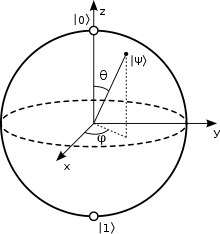
\includegraphics[scale=0.4]{bloch}\\
Рис.1 -- Кубит на сфере Блоха ~\cite{qbit}:\\

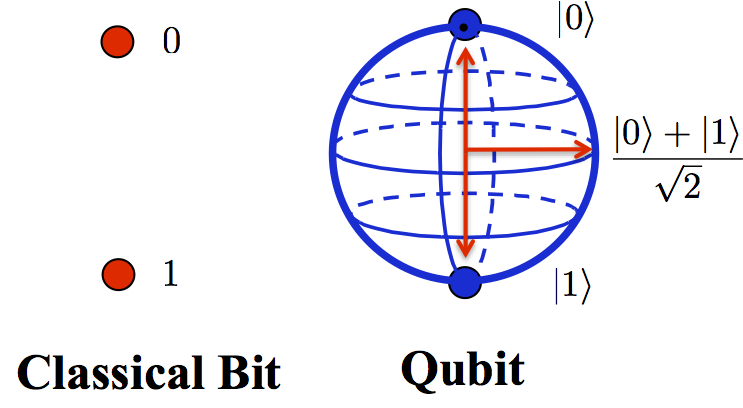
\includegraphics[scale=0.4]{qubit}\\
Зис.2 -- Кубит \\

Кубит - вектор единичной длины в двухмерном Гильбертовом пространстве над комплексными числами:\\

\begin{description}
\addtolength{\itemindent}{0.80cm}
\itemsep0em 
\item[] $H \text{ над } \mathbb{C}$
\item[] $dim(H) = 2$
\item[] $|\varphi> \in H \text{, где вектор записан в нотации Дирака} $
\item[] \text{норма} $||\varphi|| = 1$
\end{description} 
$H$ - это пространство со скалярным произведением $|x>,|y>$, где:\\
$|x> = \begin{pmatrix}
x_1 \\
\dots \\
\dots \\
x_n
\end{pmatrix}
\text{,}
|y> = \begin{pmatrix}
y_1 \\
\dots \\
\dots \\
y_n
\end{pmatrix}
\text{,}
x,y \in \mathbb{C}
$\\

Скалярное произведение $<x|y> = \sum x_i y_i^\text{*}$ \\

Пример: \\
$|x> = \begin{pmatrix}
1+i \\
e^{\pi i} \\
0 \\
1-i
\end{pmatrix}
\text{,}
|y> = \begin{pmatrix}
1+i \\
e^{2\pi i} \\
0 \\
1-i
\end{pmatrix}$\\

$<x|y>=(1+i)(1+i)+e^{\pi i}e^{2\pi i} + 0 +(1-i)^2 = 2i +e^{3\pi i} - 2i = -1
$\\

Комплексное сопряжение:

$a+bi \leftrightarrow a-bi$\\

$|y>^{\text{*}} = \begin{pmatrix}
1-i \\
e^{-2\pi i} \\
0 \\
1+i
\end{pmatrix}$\\

Косинуc угла между двух векторов будет: $cos(x,y) = \frac{|<x|y>|}{||x|| \cdot ||y||}$ \\

Угол между векторами: $\angle x,y = arccos \frac{<x|y>}{||x|| \cdot ||y||}$\\

Ортогональные вектора: $|x>|y> \rightarrow |<x|y>| = 0$\\

Сонаправленные вектора: $|x>|y> \rightarrow |<x|y>| = 1$\\

Если вектора единичные, то: $cos\alpha = <x|y>$\\

Пример:\\
$|x> \text{ и } e^{i\varphi}|x>$ - сонаправлены, но не совпадают как в Евклидовом пространстве

\section{Измерение кубита}
Кубит может принимать любое из бесконечного множества значений. Сужение количества состояний системы называется: в классической теории - оцифровка, в кванитовой - измерение.
\subsection{Выбор ортонормированного базиса}
Пусть базис выбирается наблюдателем:\\

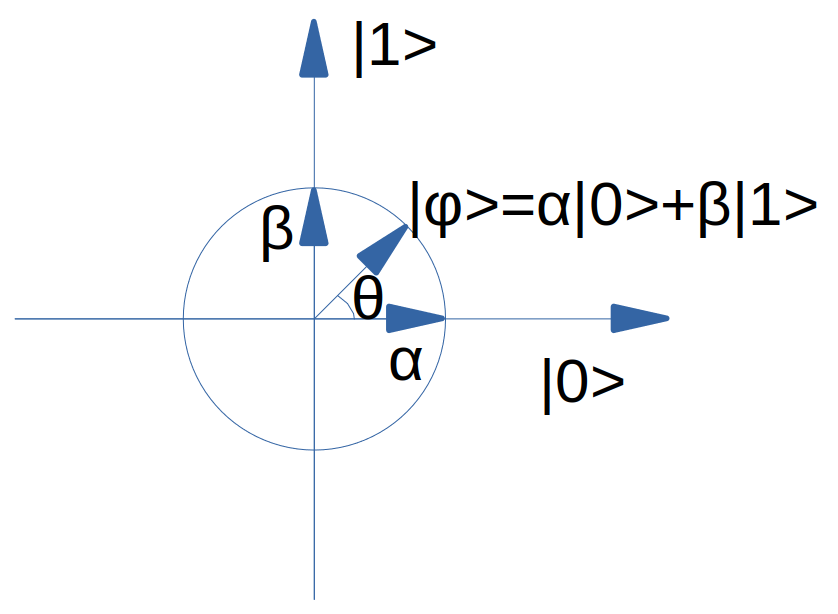
\includegraphics[scale=0.3]{basis}\\
Рис.3 -- Базис \\

$|\varphi> = |\alpha 0> +|\beta 1>\\
\alpha,\beta \in \mathbb{C}\\
|\alpha|^2+|\beta|^2=1
$ \\

При измерении вектора $|\varphi>$ в базисе $|0>|1>$ получаем:\\

$P(|0>)=|\alpha|^2$ - вероятность вектора $|0>$\\

$P(|1>)=|\beta|^2$ - вероятность вектора $|1>$\\

$\alpha =<\varphi|0>$ \\

$\beta =<\varphi|1>$ \\

$\alpha = cos\theta$ \\

$\beta = sin\theta$ \\

Определяем базис:\\
$|x>|y> : <x|y>=0, ||x||=||y||=1$ \\

\subsection{Проведение измерения}
Вероятность получения вектора $|x>$ : $P(|x>)=|<x|\varphi>|^2$, где $\varphi$ - вектор измеряемой системы, соответственно, вероятность получения вектора $|y>$ будет:\\

$P(|y>)=|<y|\varphi>|^2$.\\

\subsection{Изменение состояния системы}
Система при измерении переходит в то состояние, которое мы получили в результате измерения. Из континуума всех возможных состояний мы получаем всего 2 значения, аналогично классическому биту: $\varphi => {|x>,|y>}$ \\

$\text{квантовая информация}-\text{измерение}->\text{классическая информация}$\\

Коэффициенты $\alpha$ и $\beta$ из измерения узнать нельзя, а копировать нельзя по теореме о 
запрете клонирования.

\subsection{Базис Адамара}
Проблема:\\
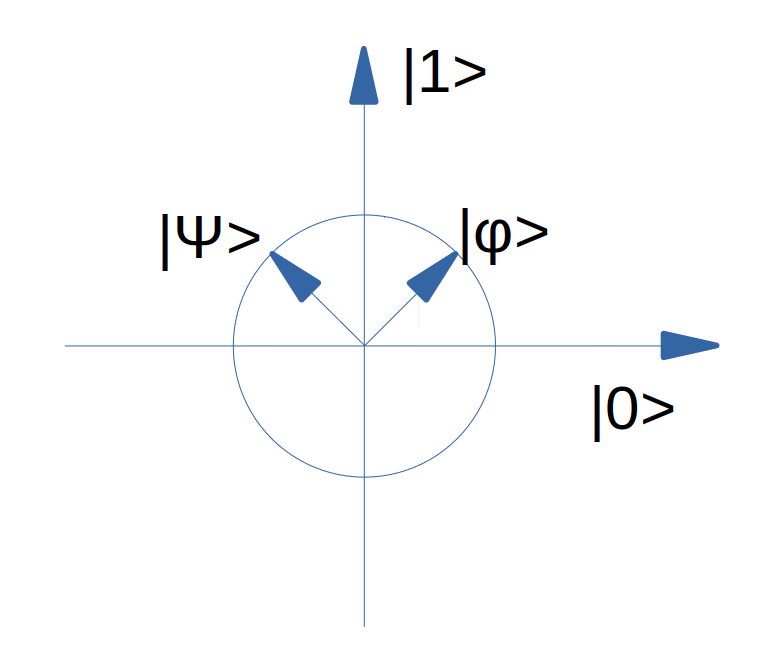
\includegraphics[scale=0.3]{adamar}\\
Рис.4 - Проблема склеивания двух векторов \\

В базисе $|0>|1>$ такой кубит измерять бесполезно, поскольку: \\

$P(|0>|\varphi) = |<\varphi|0>|^2 = \frac{1}{2} = P(|0>|\psi>)$\\

$P(|1>|\varphi) = |<\varphi|0>|^2 = \frac{1}{2} = P(|1>|\psi>)$\\

Решение проблемы в выборе нового базиса $|+>,|->$\\

$|+>=\frac{1}{\sqrt2}|0>+\frac{1}{\sqrt2}|1>$\\

$|->=\frac{1}{\sqrt2}|0>-\frac{1}{\sqrt2}|1>$\\

$P(1+>|\varphi)=|<\varphi|+>|^2$\\

Такой базис называется базисом Адамара.

\section{Система кубитов}
\subsection{Два кубита}
Систему из двух кубитов можно представить как: \\

- 2 поляризованных фотона ($\gamma$) \\

- 2 атома водорода ($p^+$) \\

- 2 $\alpha$-частицы \\

- 2 $e^-$ с разными спинами \\

В стандартном базисе:\\

\begin{tabular}{|c|c|}
\hline
	qubit1 & qubit2\\
\hline
	|0> & |0>\\
\hline
	|0> & |1>\\
\hline
	|1> & |0>\\
\hline
	|1> & |1>\\
\hline
\end{tabular}\\

Поскольку возможных результатов измерений у нас 4, то и количество базисных векторов 4 (четырех мерное пространство)\\

\begin{tabular}{|c|c|c|}
\hline
	qubit1 & qubit2 & вектор\\
\hline
	|0> & |0> & |00> \\
\hline
	|0> & |1> & |01> \\
\hline
	|1> & |0> & |10> \\
\hline
	|1> & |1> & |11> \\
\hline
\end{tabular} \\

До измерения:\\

$|0> : \alpha |0> \beta |1>$ \\

что соответствует: \\

$|0> : \alpha |00> + \beta |01>$ \\

Вероятность измерения векторов будет: \\

$P(|00>) = |\alpha|^2$ \\

$P(|01>) = |\beta|^2$ \\

$P(|10>) = P(|11>) = 0$ \\


Полностью смешанное состояние: \\

\begin{tabular}{|c|c|c|}
\hline
	qubit1 & qubit2 & вектор\\
\hline
	$\alpha|0> + \beta|1>$ & $\gamma|0> + \delta|1>$ & | $\alpha \gamma |0> + \alpha \delta|01> + \beta \gamma |10> + \beta\delta|11>$ \\
	\hline
\end{tabular}\\

Любой вектор в пространстве $H^{2^n}$ представляет собой какое-то реально возможное состояние из n кубитов\\ 

Пример:\\

Рассмотрим вектора $|0>=\begin{pmatrix}
1 \\
0
\end{pmatrix}$ 
и 
$|1>=\begin{pmatrix}
0 \\
1
\end{pmatrix}$ \\

Для двух и более кубитов используется тензорное (кронекерово) произведение:\\

$|00> = \begin{pmatrix}
1 \\
0
\end{pmatrix}
\otimes
\begin{pmatrix}
0 \\
1
\end{pmatrix}
=
\begin{pmatrix}
1 \begin{pmatrix}1 \\
0\end{pmatrix} \\
0 \begin{pmatrix}1 \\
0\end{pmatrix}
\end{pmatrix} =
\begin{pmatrix}
1 \\
0 \\
0 \\
0 \\
\end{pmatrix}$ \\

$|01> = \begin{pmatrix}
1 \\
0
\end{pmatrix}
\otimes
\begin{pmatrix}
0 \\
1
\end{pmatrix}
=
\begin{pmatrix}
1 
\begin{pmatrix}
0 \\
1\end{pmatrix} \\

0 
\begin{pmatrix}
0 \\
1\end{pmatrix}

\end{pmatrix} =
\begin{pmatrix}
0 \\
1 \\
0 \\
0 \\
\end{pmatrix}$ \\

$|10> = \begin{pmatrix}
0 \\
1
\end{pmatrix}
\otimes
\begin{pmatrix}
1 \\
0
\end{pmatrix}
=
\begin{pmatrix}
0 
\begin{pmatrix}
1 \\
0\end{pmatrix} \\

1 
\begin{pmatrix}
1 \\
0\end{pmatrix}

\end{pmatrix} =
\begin{pmatrix}
0 \\
0 \\
1 \\
0 \\
\end{pmatrix}$

$|11> = \begin{pmatrix}
0 \\
1
\end{pmatrix}
\otimes
\begin{pmatrix}
0 \\
1
\end{pmatrix}
=
\begin{pmatrix}
0 
\begin{pmatrix}
0 \\
1\end{pmatrix} \\

1 
\begin{pmatrix}
0 \\
1\end{pmatrix}

\end{pmatrix} =
\begin{pmatrix}
0 \\
0 \\
0 \\
1 \\
\end{pmatrix}$
\subsection{N кубитов}
Система из 3q описывается векторами в $2^3 = 8$ми мерном пространстве. Размерность системы из $10q=2^{10} = 1024$

\section{Измерение системы кубитов}
Не любое состояние вида: \\

$\alpha|00>+\beta|01>+\gamma|10>+\delta|11>$\\

$|\alpha|^2 + |\beta|^2 + |\gamma|^2 + |\delta|^2 = 0$ \\

раскладывается на тензорное произведение отдельных кубитов.\\

Запишем тензорное произведение двух кубитов находящихся в состоянии суперпозиции: \\

$(\alpha|0>+\beta|1>)(\gamma|0>+\delta|1>) = \alpha \gamma |00> + \alpha \delta |01> +\beta \gamma |10> +\beta \delta |11>$ \\

данное произведение описывает состояние какой-то реально существующей системы, например: \\

$\frac{1}{\sqrt2}(|00>+|11>)$ - одно из состояний Бэлла, для которого нельзя сделать разложение. Получается для каждой отдельной частицы, составляющих это состояние нет своего персонального состояния. Эти частицы запутаны.\\

Пусть мы измерили в общем случае первый кубит и получили в качестве результата $|0>$, то второй кубит у нас остается и равен $(\gamma|0>+\delta|1>)$, т.е. при измерении первого кубита, второй кубит остается целым и результат его измерения по прежнему не определен. \\

Для состояния Бэлла, если мы измерили первый кубит и получили $|0>$ то второй кубит вынужден быть $|0>$, т.е. $|0>|0>=|00> $. Получается, что измерение первого кубита однозначно определяет второй кубит, при том, что до измерения первого кубита, второй кубит не находился в этом конкретном состоянии.\\

\section{Эволюция квантовой системы}
Поскольку изменение состояния и есть вычисление, то и "программа" для квантового компьютера представляет собой последовательное применение в векторе $|\dots>$ различных U-унитарных операторов 
$UU^{*}=U^{*}U=I$, такого, что его сопряженный оператор совпадает с обратным.

\subsection{Оператор Адамара}
Из стандартного базиса оператор Адамара создает базис Адамара: \\

$H|0>=\frac{1}{\sqrt2}\begin{pmatrix}
1 && 1 \\
1 && -1\end{pmatrix}
\begin{pmatrix}
1 \\
0\end{pmatrix}
= \frac{1}{\sqrt2}
\begin{pmatrix}
1 \\
1\end{pmatrix}
=|+>$ \\

$H|1>=\frac{1}{\sqrt2}\begin{pmatrix}
1 && 1 \\
1 && -1\end{pmatrix}
\begin{pmatrix}
0 \\
1\end{pmatrix}
= \frac{1}{\sqrt2}
\begin{pmatrix}
1 \\
-1\end{pmatrix}
=|->$ \\


\subsection{Гейт X}
Квантовый аналог классического NOT\\

$X=\begin{pmatrix}
0 && 1 \\
1 && 0\end{pmatrix}
$\\

$X^{*}=X$\\

$XX=\begin{pmatrix}
0 && 1 \\
1 && 0\end{pmatrix} 
\begin{pmatrix}
0 && 1 \\
1 && 0\end{pmatrix} 
=
\begin{pmatrix}
0\cdot0+1\cdot1 && 0\cdot 1 + 1 \cdot 0\\

1\cdot 0 + 0 \cdot 1 && 1\cdot 1 + 0 \cdot 0\end{pmatrix}= \\=
\begin{pmatrix}
1 && 0 \\
0 && 1\end{pmatrix}=I$

\subsection{Гейт CNOT}
На схемах гейт изображается следующим образом: \\

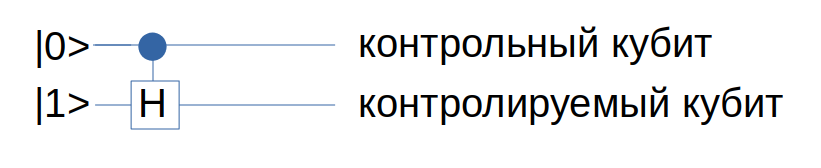
\includegraphics[scale=0.3]{cnot}\\
Рис.5 - Оператор CNOT\\

Имеет вид:\\

$
\begin{pmatrix}
1 && 0 && 0 && 0 \\
0 && 1 && 0 && 0 \\
0 && 0 && 0 && 1  \\
0 && 0 && 1 && 0
\end{pmatrix}
$ \\

"смотрит" на первый бит, если 1, то применяет NOT ко второму биту: \\

$CNOT|00>=|00>$ \\

$CNOT|01>=|01>$ \\

$CNOT|10>=|11>$ \\

$CNOT|11>=|10>$ \\


\section{Схема квантового алгоритма}
\subsection{Применение оператора Адамара сразу к двум кубитам} 
Рассмотрим схему: \\

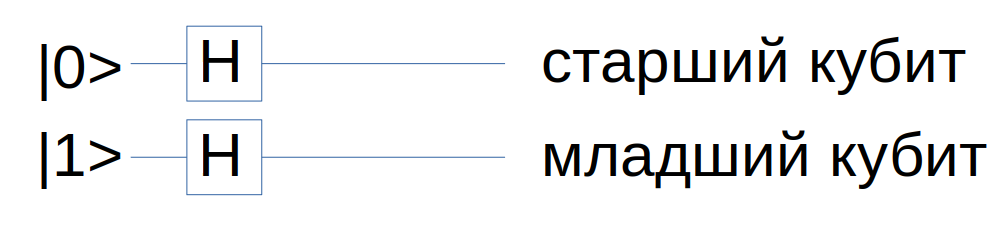
\includegraphics[scale=0.2]{shema}\\
Рис.6 -- Применение оператора Адамара сразу к двум кубитам\\

запишем в виде: \\

$H_2 = H\otimes H = \frac{1}{\sqrt2}\begin{pmatrix}
1 && 1 \\
1 && -1\end{pmatrix} \otimes
\frac{1}{\sqrt2}\begin{pmatrix}
1 && 1 \\
1 && -1\end{pmatrix} = \frac{1}{2}\begin{pmatrix}
H && H \\
H && -H\end{pmatrix} = \frac{1}{2}\begin{pmatrix}
1 && 1 && 1 && 1 \\
1 && -1 && 1 && -1 \\
1 && 1 && -1 && -1 \\
1 && -1 && -1 && 1\end{pmatrix}$\\

Двухкубитный оператор Адамара - это тензорное произведение однокубитных:\\

$A|x> \otimes B|y> = (A\otimes B) | xy>$

\subsection{Адамар на младшем кубите}
Рассмотрим схему Адамара на младшем кубите: \\

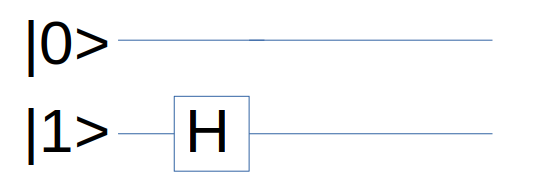
\includegraphics[scale=0.2]{adamar_ml}\\
Рис.7 -- Адамар на младшем кубите \\

Поскольку с первым кубитом ничего не происходит, то это равносильно применению к нему тождественного оператора:\\

$I\otimes H = \frac{1}{\sqrt2}\begin{pmatrix}
1 && 0 \\
0 && 1\end{pmatrix} \begin{pmatrix}
1 && 1 \\
1 && -1\end{pmatrix} = \begin{pmatrix}
H && 0 \\
0 && H \end{pmatrix} = 
\frac{1}{\sqrt2}\begin{pmatrix}
1 && 1 && 0 && 0  \\
1 && -1 && 0 && 0 \\
0 && 0 && 1 && 1 \\
0 && 0 && 1 && -1
 \end{pmatrix}$
 
\subsection{Адамар на старшем кубите}
Разберем вариант Адамара на старшем кубите: \\

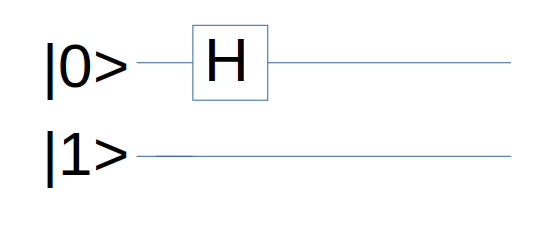
\includegraphics[scale=0.2]{adamar_st}\\
Рис.8 -- Адамара на старшем кубите \\

запишем: \\

$H\otimes I = \frac{1}{\sqrt2}\begin{pmatrix}
1 && 1 \\
1 && -1\end{pmatrix} 
\begin{pmatrix}
1 && 0 \\
0 && 1\end{pmatrix} = \frac{1}{\sqrt2}\begin{pmatrix}
1 && 0 && 1 && 0 \\
0 && 1 && 0 && 1 \\
1 && 0 && -1 && 0 \\
0 && 1 && 0 && -1\end{pmatrix}$

\subsection{Оператор CNOT в 3q системах}
Примеры CNOT в 3q системах: \\

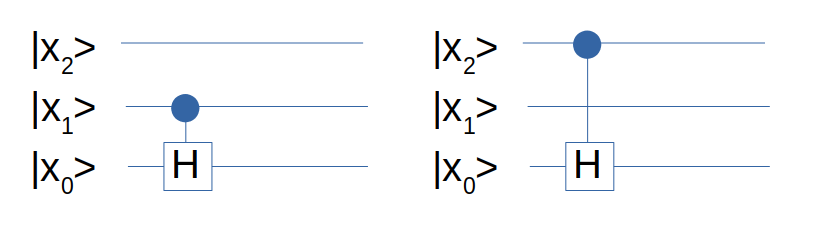
\includegraphics[scale=0.3]{cnot_3}\\
Рис.9 -- Примеры CNOT в 3q системах \\

CNOT запутывающий оператор и с помощью его получают запутанные состояния. \\

В общем виде действие оператора можно представить:\\

$A_{ek} = \begin{pmatrix}
a_{11} && a_{12} && \dots && a_{1k} && a_{1n} \\
a_{21} && a_{22} && \dots && a_{2k} && a_{2n} \\
\dots && \dots && \dots && \dots && \dots \\
a_{n1} && a_{n2} && \dots && a_{nk} && a_{nn} \\
\end{pmatrix}\cdot \begin{pmatrix}
0  \\
\dots \\
1 \\
0 \\
 \end{pmatrix} = \begin{pmatrix}
 a_{1k} \\
 a_{2k} \\
 \dots \\
a_{nk}
 \end{pmatrix}$ \\

Распишем варианты оператора с контрольным $x_2$ кубитом: \\

$|000> \rightarrow |000>$ \\

$|001> \rightarrow |001>$ \\

$|010> \rightarrow |010>$ \\

$|011> \rightarrow |011>$ \\

$|100> \rightarrow |100>$ \\

$|101> \rightarrow |100>$ \\

$|110> \rightarrow |111>$ \\

$|111> \rightarrow |110>$ \\

Матричная форма оператора: \\

$\begin{pmatrix}
1&&0&&0&&0&&0&&0&&0\\
0 && 1 && 0 && 0 && 0 && 0 && 0 \\
0 && 0 && 1 && 0 && 0 && 0 && 0 \\
0 && 0 && 0 && 1 && 0 && 0 && 0 \\
0 && 0 && 0 && 0 && 1 && 0 && 0 \\
0 && 0 && 0 && 1 && 0 && 0 && 0 \\
0 && 0 && 0 && 0 && 0 && 0 && 1 \\
0 && 0 && 0 && 0 && 0 && 1 && 0 \end{pmatrix}$

\subsection{Оператор Адамара в Nq системах}
Оператор Адамара в Nq системах описывается выражением: \\

$H_n|x> = \frac{1}{2^{n/2}}\sum\limits_{y=0}^{2^n-1} (-1)^{x\bullet y}|y>$ , где: \\

$x\bullet y = x_0y_0 \bigoplus x_1y_1 \bigoplus \dots x_{n-1}y_{n-1}$


\section{Задача Дойча}
Имеем черный ящик с функцией $f$, которая может быть:\\

$f(x) = 0$ \\

$f(x) = 1$ \\

$f(x) = x$ \\

$f(x) = \bar{x} $, где $x$ принимает значения \{\ 0,1 \}\ и результат, возвращаемый из функции есть \{\ 0,1 \}\ \\

В классике, нужно вызвать функцию $f(x)$ два раза, чтобы ответить на вопрос является ли функция константой. Но на квантовом компьютере достаточно одного вызова. \\

Квантовый компьютер, реализующий данный алгоритм мы и будем реализовывать на стендах. \\

Разберем теоретическое решение задачи. \\

Так как эволюция квантовой системы унитарна, то вместо $f(x)$ в черном ящике должен быть реализован унитарный оператор $U_f$, который в отличии от $f(x)$ должен быть обратим:\\

$U_f|x>|y> = |x>|y+f(x)>$, где \\

$U_f$ - работает с двумя кубитами, а $f(x)$ с одним битом.\\

В векторе $|x>$ будем хранить первообраз $f(x)$ для обратимости и этот кубит не должен затрагиваться действием оператора, тогда: \\

$U_f|0>|0> \rightarrow |0>|f(0)$ \\

$U_f|1>|0> \rightarrow |1>|f(1)$  \\

При этом нельзя допустить "склеивания" векторов: \\

$U_f|0>|1> \rightarrow |0>|1 \bigoplus f(0)> \neq |0>|f(0)> = U_f|0>|0> $ \\

$U_f|1>|1> \rightarrow |1>|1 \bigoplus f(1)> \neq |1>|f(1)> = U_f|1>|0> $ \\

Проверим как $U_f$ действует на $|x>(|0>-|1>)$ : \\

$U_f\frac{1}{\sqrt2}|x>(|0>-|1>)=\frac{1}{\sqrt2}|x>(|0 \bigoplus f(x)> - |1 \bigoplus f(x)>) \\ = 
\frac{1}{\sqrt2}(-1)^{f(x)}|x>(|0>-|1>)$ \\

из чего видно, что если $f(x)=1$ то $x$ домножается на -1 \\

$U_f|x>|y> = |x>|y + f(x)$>

\subsection{Вариант $f(x)=0$}
При варианте $f(x)=0$ действие оператора $U_f$ будет: \\

$U_f|x>|y> = |x>|y>$  \\

, следовательно $U_f = I$ \\

Таким образом с кубитами ничего не происходит:  \\

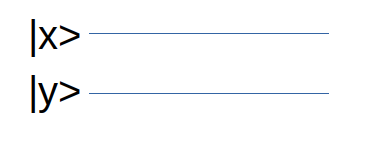
\includegraphics[scale=0.3]{f_0}\\
Рис.10 -- С кубитами ничего не происходит\\

\subsection{Вариант $f(x)=1$}

Рассмотрим вариант $f(x)=1$: \\

$U_f|x>|y> = |x>|y \bigoplus 1 >$ \\

Возможные состояния векторов будут: \\

$|00> \rightarrow |01> $ \\

$|01> \rightarrow |00> $ \\

$|10> \rightarrow |11> $ \\

$|11> \rightarrow |10> $ \\

следовательно: \\

$U_f = \begin{pmatrix}
0 && 1 && 0 && 0 \\
1 && 0 && 0 && 0 \\
0 && 0 && 0 && 1 \\
0 && 0 && 1 && 0 \\
\end{pmatrix} = I \otimes X$\\

, что соответствует следующей схеме: \\

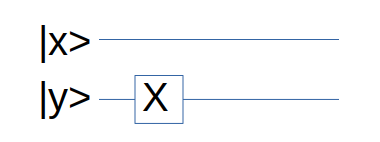
\includegraphics[scale=0.3]{f_1}\\
Рис.11 -- схема при f(x)=1\\

\subsection{Вариант $f(x)=x$}
Оператор $U_f$ будет в этом случае работать следующим образом: \\

$U_f|x>|y>=|x>|y \bigoplus x> $ \\

, тогда вектора будут изменяться: \\

$|00> \rightarrow |00> $ \\

$|01> \rightarrow |01> $ \\

$|10> \rightarrow |11> $ \\

$|11> \rightarrow |10> $ \\

, что соответствует поведению CNOT:\\

$U_f = CNOT = \begin{pmatrix}
1 && 0 && 0 && 0 \\
0 && 1 && 0 && 0 \\
0 && 0 && 0 && 1 \\
0 && 0 && 1 && 0 \\
\end{pmatrix}$

и так будет выглядеть на схеме:\\

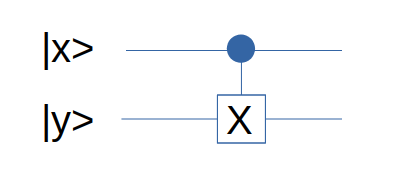
\includegraphics[scale=0.3]{f_x} \\
Рис.12 -- схема при f(x)=x\\

\subsection{Вариант $f(x) = \bar{x} $}
Варианты изменения векторов будут: \\

$|00> \rightarrow |01> $ \\

$|01> \rightarrow |00> $ \\

$|10> \rightarrow |10> $ \\

$|11> \rightarrow |11> $ \\

, тогда: \\

$U_f = \begin{pmatrix}
0 && 1 && 0 && 0 \\
1 && 0 && 0 && 0 \\
0 && 0 && 1 && 0 \\
0 && 0 && 0 && 1 \\
\end{pmatrix}$ \\

и будет представлен на схеме как: \\

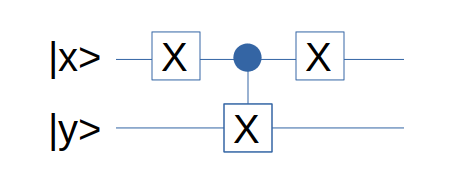
\includegraphics[scale=0.3]{f_not_x}
Рис.13 -- схема при f(x)/=1\\

\subsection{Алгоритм Дойча}
На схеме алгоритм Дойча изображается: \\

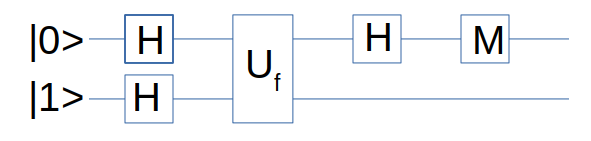
\includegraphics[scale=0.3]{doych}\\
Рис.14 -- алгоритм Дойча\\

, где M - измерение \\

На вход подаем состояние $|0>|1>$ и применяем к нему оператор Адамара:\\

$\frac{1}{2}(|0>+|1>)(|0>-|1>) = \frac{1}{2}|0>(|0>-|1>)+\frac{1}{2}|1>(|0>-|1>)$ \\

затем применяем оператор $U_f$: \\

$\frac{1}{2}(-1)^{f(0)}|0>(|0>-|1>) + \frac{1}{2}(-1)^{f(1)}|1>(|0>-|1>) = \\
\frac{1}{2}((-1)^{f(0)}|0> + (-1)^{f(1)}|1>)(|0>-|1>)
$ \\

Затем, перед повторным применением оператора Адамара, разберем случаи: \\

\begin{description}
\addtolength{\itemindent}{0.80cm}
\itemsep0em 
\item[$f(x)=const$]: $\pm \frac{1}{2}(|0> + |1>) = \pm H(|0>) = |0> $
\item[$f(0) \neq f(1) $]: $\pm \frac{1}{2}(|0> + |1>) = \pm H(|1>) = |1>$ \\

Таким образом видно, что за один "проход" подавай на вход $|0>|1>$ и получая на выходе $|0>$ мы узнаем, что $f(x)=const$, и если результат равен $|1>$, то функция сбалансирована.

\end{description}

\chapter{Физическая реализация квантового оператора}
\section{Обзор}
Квантовые операторы хорошо представлены в сводной таблице~\cite{qbit}: \\

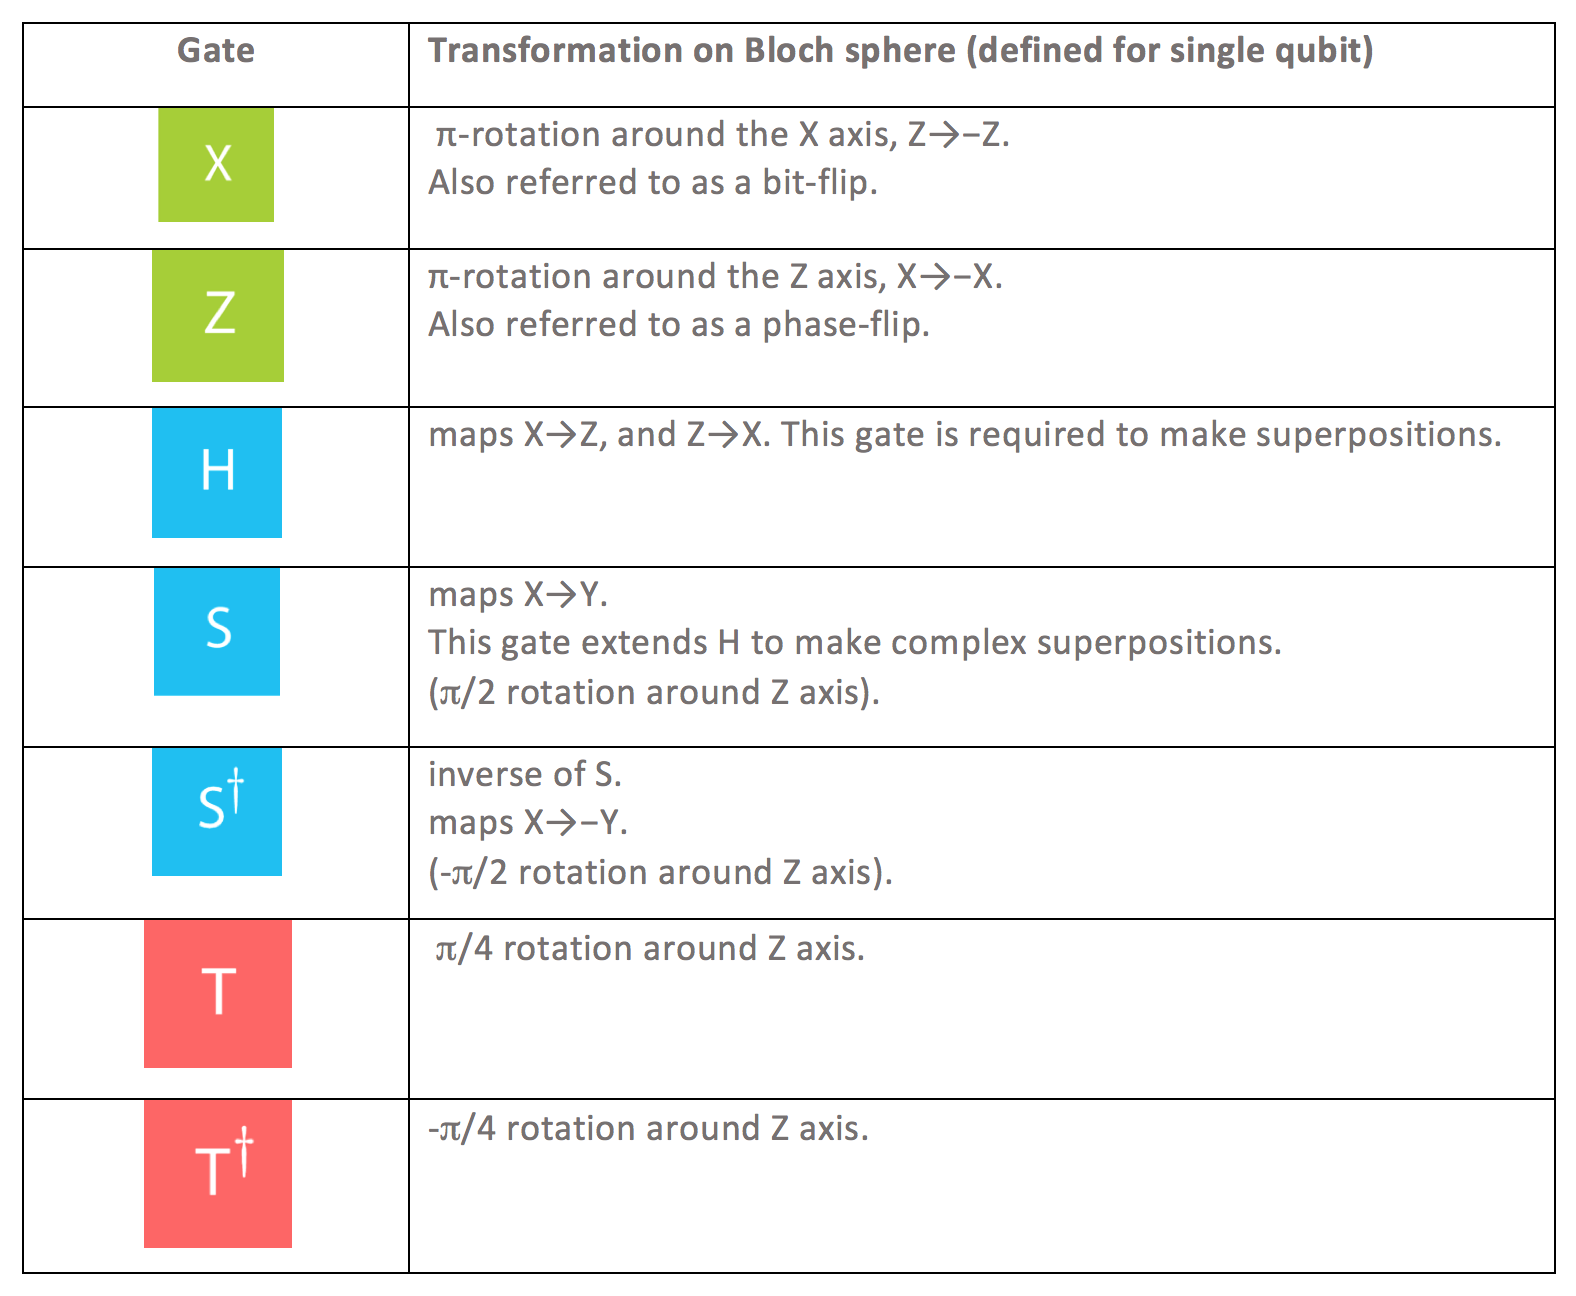
\includegraphics[scale=0.2]{operators} \\
Рис.15 -- Квантовые операторы \\

На текущий момент не принципиально, что делает конкретный оператор, главное определить принцип его работы, а он с математической точки зрения - изменение радиус вектора на комплексной сфере, а с физической - процесс, при котором изменяется вектор в пространстве-времени, который мы выбрали в качестве вектора суперпозиции кубита. Оператор кроме описанной выше векторной нотации мы можем представить диаграммой Феймана, как и весь процесс вычисления целиком. \\

Для идентификации элементарной частицы необходимо знать ~\cite{saricheva}:
\begin{description}
\addtolength{\itemindent}{0.80cm}
\itemsep0em 
\item[] $I $ - изотопический спин;
\item[] $J $ - собственный момент количества движения - спин;
\item[] $P $ - пространственную четность;
\item[] $C $  - зарядовую четность;
\item[] $G $ - G-четность;
\end{description} 

Также для описания явления используется:
\begin{description}
\addtolength{\itemindent}{0.80cm}
\itemsep0em 
\item[R] 4-вектор  пространство-время
\item[M] масса
\item[Q] заряд электрический
\item[E] энергия
\item[J] спин
\item[S] орбитальный момент
\item[$\mu$] магнитный момент
\item[B] барионное число
\item[L] лептонное число
\item[C] аромат
\end{description}

Учитываются четыре типа взаимодействий:\\
\begin{description}
\addtolength{\itemindent}{0.80cm}
\itemsep0em
\item[] - электромагнитное
\item[] - слабое,
\item[] - сильное 
\item[] - гравитационное
\end{description}


Диаграммы Фейнмана, отображают харктер взаимодействия и соблюдают законы сохранений (энергии, импульса, заряда, барионного числа, лептонного числа, аромата(за исключением заряженных слабых взаимодействий)), что важно для квантовых вычислений. \\

Квантовые операторы могут быть записаны некоторой последовательностью диаграмм Фейнмана, либо одной диаграммой, на которой действие оператора будет характеризоваться виртуальной частицей (бозонов).

Свойства фундаментальных бозонов ~\cite{saricheva}:\\
\begin{tabular}{|p{6cm}|p{2cm}|p{2cm}|p{4cm}|}
\hline
	Название  & Заряд & Спин & Взаимодействие \\
\hline	
	Гравитон  & 0 & 2 & Гравитационное \\
\hline
	Фотон     & 0 & 1 & Электромагнитное \\
\hline
	Заряженные векторные бозоны, $W^{\pm}$     & $\pm$1 & 1 & Слабое \\	
\hline
	Нейтральный векторный бозон, $Z^0$     & 0 & 1 & Слабое \\		
\hline
	Глюоны, $g_1,\dots,g_8$     & 0 & 0 & Сильное \\			
\hline
	Хиггсы, $H^0,H^{\pm}$     & 0 & 0 &  \\				
\hline	
\end{tabular}\\

Пример диаграммы Фейнмана: \\
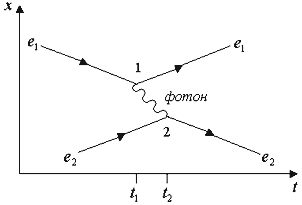
\includegraphics[scale=1]{feinman}
Рис.16 -- Диаграмма Фейнмана \\

Из наиболее вероятных процессов в нашем рассмотрении - будут процессы рассеивания.
\section{Процесс рассеивания}
Процесс рассеивания характеризуется сечением рассеивания: \\

$\frac{-dI}{I} = \sigma n$, \\

где $n$ - поверхносная плотность рассеивателей, \\

$I$ - интенсивность потока частиц. \\

Измерив изменение интенсивности, мы можем рассчитать сечение, и наоборот, зная сечение, мы можем предсказать изменение интенсивности. Этот факт будет являться основой для получения результатов рассчета из квантового компьютера на классический.\\

$\sigma_{tot} = \sigma_{el}+\sigma_{inel}+\sigma_{abs}$\\

Полное поперечное сечение состоит из сечения упругого рассеяния, неупругого рассеяния и поглощения.\\

Коэффициент пропорциональности между скоростью счета и поперечным сечением называется светимостью - L.\\

\section{Заключение}
Квантовые операторы возможно представить в виде диаграмм Фейнмана. Основное рассматриваемое событие - рассеивание. Рассеивание характеризуется сечением. Сечение можно определить по изменению интенсивности, свечению. \\

Таким образом было построено полное соответствие между двумя дисциплинами - квантовыми вычислениями и ядерной физикой. \\

Следующей задачей будет найти физические аналоги кванотовым алгоритмам и физические(квантовые) события - квантовым операторам. \\

\chapter{Физические основы квантовых вычислений}

\section{Квантовые интерференционные картины}
 Любое измерение квантовой величины можно рассматривать как процесс выделения некоторого количества собственных значений $a_i$ из спектра данной физической величины А. При выделении полосы конечной ширины $c=\Delta a$ из непрерывного во всей бесконечной области спектра собственных значений оператора $A$ наблюдается определенная интерференционная картина в распределении интенсивности в спектре собственных значений оператора $B$ сопряженной наблюдаемой величины, коммутатор которого с оператором $A$ определяется выражением:\\
 
 $[A,B] = i\hbar$ \\
 
 Например, координата и импульс $[x,p_x]$, когда выделение области $\Delta x$ обуславливает возникновение дифракционной картины шириной $\Delta p_x \gtrsim \frac{\hbar}{\Delta x}$ для сопряженной величины импульса. Квантовая дифракция не ограничена этим простейшим случаем. Она наблюдается для любой пары величин $A$ и $B$ и соотношение неопределенностей для их дисперсий будет: \\

 $<(\Delta A)^2><(\Delta B)^2> \gtrsim \frac{1}{4}\hbar^2$ \\

 В квантовой механике дифракционные явления наблюдаются для любых пар сопряженных физических величин, если область $C$ содержит достаточно большое число собственных значений $a_i$. Это относится к операторам, имеющим дискретный спектр, который можно считать квазинепрерывным в том смысле, что амплитуды и фазы волновых функций сильно размыты по области $C$ - это случай больших квантовых чисел, т.е. он соответствует квази классическому пределу, например, коммутационное соотношение угла и орбитального момента: \\
 
  $[\varphi,l_z] = i\hbar$ \\
  
  а соотношение неопределенностей, равное: \\
  
$<(\Delta \varphi)^2><(\Delta l_z)^2> \gtrsim \frac{1}{4}\hbar^2$ \\

не строго точно, так как спектр оператора $l_z$ дискретный и ограниченный, но для больших собственных значений $ l_i \gg \hbar$ спектр оператора $l_z$ можно рассматривать как квазинепрерывный (квазиклассический случай), т.е. обычная форма соотношения неопределенностей является хорошим приближением. Такая ситуация имеет место в области высоких энергий для многих процессов взаимодействия, когда рассеиватель сильно поглощает бомбардирующие частицы, а его характерный размер велик по сравнению с длиной волны налетающей частицы. \\

Еще один пример - интерференционная картина дифракции в представлении прицельного параметра, также рассматриваемая в области высоких энергий. В этом случае сопряженной переменной для прицельного параметра будет переданный импульс. Разновидностью представления прицельного параметра является приближение эйконала. \\

Если квантовое измерение определяется проекционным оператором: \\

$T = \int_C|a' > da' < a'|$ \\

то изменение вектора состояния |$\psi$> в $a$-представлении в результате измерения $T$ равно: \\

$<a|\psi>_C = <a|T|\psi> = \int_C da'<a|a'><a'|\psi>$ \\

Произведенное измерение $T$ изменяет также волновую функцию в $b$-представлении: \\

$<b|\psi>_C = <b|T|\psi> = \int_C da'<b|a'><a'|\psi>$ \\
  
Интерференционная картина в $b$-пространстве определяется интенсивностью: \\
  
$I_C(b) = |<b|\psi>_C|^2$ . \\

Собственная функция $<b|a>$ будет:\\

$<b|a> =\frac{1}{\sqrt 2 \pi \hbar} e^{-\frac{iab}{\hbar}}$

Выделяем в волновой функции $<a|\psi>$ амплитуду $\eta(a) $ и фазу $\Omega(a)$ : \\

$<a|\psi> = \eta(a)e^{\frac{i\Omega(a)}{\hbar}}$ \\

получаем выражение для волновой функции $<b|\psi>_C$: \\

$<b|\psi>_C = \frac{1}{\sqrt 2 \pi \hbar} \int_C da \eta(a) e^{\frac{i}{\hbar}(\Omega(a) - ab)}$

По аналогии с основным предположением классической оптики теории дифракции следует полагать, что фаза $\Omega(a)$ медленно меняется в области $C=\Delta a$, а значит ее можно разложить в ряд окрестности точки $a_0$ , находящейся в области $C$ : \\ 

$\Omega(a) = \Omega(a_0)+(a-a_0)\Omega'(a_0)+\frac{1}{2}(a-a_0)^2\Omega''(a_0)+\frac{1}{6}(a-a_0)^3\Omega'''(a_0) + \dots$ \\

Если в данном разложении основную роль играет: \\

\begin{description}
\addtolength{\itemindent}{0.80cm}
\itemsep0em 
\item[$(a-a_0)\Omega'(a_0)$] - будет наблюдаться дифракционная картина, аналогичная дифракции Фраунгофера(или дифракция плоских световых волн, или дифракция в параллельных лучах)) в оптике
\item[$\frac{1}{2}(a-a_0)^2\Omega''(a_0)$ ] - аналог оптической дифракции Френеля
\item[$|\Omega''(a_0)| \ll |\Omega'(a_0)| \text{и} |\Omega''(a_0)| \ll |\Omega'''(a_0)|$] - если кубический член того же порядка, что и линейный, то возникает картина радужного рассеяния, являющаяся интерференционной картиной, а не дифракционной. 
\end{description}

\subsection{Аналог дифракции Фраунгофера}
Рассмотрим первый случай: \\

$<b|\psi>_C=\frac{1}{sqrt 2 \pi \hbar}e^{\frac{i}{\hbar}(\Omega(a_0)-a_0b_0)}\int_Cda\eta_C(a)e^{-\frac{i}{\hbar}(b-b_0)a}$, где: \\

$b_0=\Omega'(a_0)$\\

$\eta_C(a)$ - амплитуда волновой функции $<a|\psi>_C$\\

Видим, что это соответствует преобразованию Фурье от амплитуды $\eta_C(a)$ с точностью до фазового множителя\\

\subsection{Аналог дифракции Фраунгофера от одной длинной и узкой щели}
Рассмотрим дифракцию Фраунгофера от одной длинной и узкой щели шириной $2\delta$, середина которой определяется величиной $ a_0 $ при этом амплитуда $\eta_C(a)$ предполагается постоянной в области щели $C=2\delta$:  \\

$
\eta_C(a) =
\left\{
\begin{array}{lr}
\eta_0 & \text{,}-\delta \leq a \leq \delta \\
0 & \text{,} a < -\delta, a>\delta
\end{array}
\right.
$ \\

, тогда: \\

$<b|\psi>_C=\frac{2\eta_0\delta}{\sqrt2\pi\hbar}e^{\frac{i}{\hbar}(\Omega(a_0)-a_0b_0)}\frac{sin\pi\xi}{\pi\xi}$, где \\

$\xi = \frac{(b-b_0)\delta}{\pi\hbar}$ \\

$I_C(b)=I_C(b_0)(\frac{sin\pi\xi}{\pi\xi})^2$ , $I_C(b_0)=\frac{2|\eta_0|^2\delta^2}{\pi \hbar }$- интенсивности.

\subsection{Аналог дифракции Фраунгофера от круглого отверстия}
Рассмотрим дифракцию Фраунгофера от круглого отверстия радиуса $R$. при этом волновая функция будет двумерной $<a_1a_2|\psi>_C$, и предполагается, что она постоянна в области отверстия: \\

$
<a_1a_2|\psi>_C =
\left\{
\begin{array}{lr}
\eta_0e^{i\Omega_0} & \text{,}-\rho \leq R, \\
0 & \text{,} \rho> R,
\end{array}
\right.
$ где $\rho=\sqrt{a_1^2+a_2^2}$.\\

Переходим к полярным координатам: \\ 

$a_1 = \rho cos \varphi $, \\

$a_2 = \rho sin\varphi $, \\

$b_1 = b cos \chi $, \\

$a_2 = b sin\chi $\\

$<b_1b_2|\psi>_C = \frac{\eta_0e^{i\Omega_0}}{2pi\hbar}\int_0^Rd\rho\rho \int_0^{2\pi}d\varphi e^{-\frac{i}{\\hbar}\rho b cos(\varphi - \chi)} = \frac{R^2\eta_0e^{i\Omega_0}}{\hbar} \frac{J_1(Rb/\hbar)}{Rb/\hbar }$\\

Получаем для интенсивности картину Эйри для дифракции Фраунгофера от круглого отверстия:\\

$I_C(b) = I_C(0)(\frac{2J_1(Rb/\hbar)}{Rb/\hbar})^2$ , $I_C(0) = \frac{|\eta_0|^2R^4}{4\hbar^2 }$ \\



\subsection{Аналог дифракции Френеля от края полуплоскости}
Пусть $a_0 \leq a < ∞$, тогда основной вклад в формулу разложения дает окрестность точки стационарной фазы $a_s \in C$, определяемой из условия: \\

$\omega'(a_s)=b $. \\

Если точка $a_s$ существует, то разложение фазы вблизи этой точки с точностью до членов второго порядка по $a$ (предполагается, что $\Omega''(a_s)\neq0 $ ) имеет вид: \\

$\Omega(a) = \Omega(a_s) + (a-a_s)b + \frac{1}{2}(a-a_s)^2\Omega''(a_s)$ \\

тогда: \\

$<b|\psi>_C = \frac{\eta(a_s)}{\sqrt{2\pi \hbar}}e^{\frac{i}{\hbar}(\Omega(a_s)-a_sb)}\int_{-∞}^{a_0}dae^{\frac{i\Omega''(a_s)}{2\hbar}(a-a_s)^2} $ \\

затем делаем замену переменной: \\

 $a=a_s-e^{\frac{i\pi}{4}}\sqrt{\frac{2\hbar}{\Omega''(a_s)}}t$ \\
 
 и получаем: \\

$<b|\psi>=\frac{\eta(a_s)}{2\sqrt{\Omega''(a_s)}}e^{i\tau}erfc(e^{-frac{i\pi}{4}}\sqrt{\frac{\Omega''(a_s)}{2\hbar}}(a_s-a_0)) $, где: \\

$ erfc(z)= \frac{2}{\sqrt\pi\int_z^∞dte^{-t^2}}$ \\

$\tau = (\frac{i}{\hbar})(\Omega(a_s) -a_sb) + \frac{i\pi }{4} $ \\

используем соотношения:\\

$\Omega'(a_s) \approx \Omega'(a_0) + (a_s-a_0)\Omega''(a_0) $ \\

$\Omega'(a_s) =b $ \\

$\Omega'(a_0) =b_0 $ \\

получаем: \\

$a_s = a_0+\frac{b-b_0}{\Omega''(a_0)}$ \\

 и так как:\\
 
  $\Omega''(a_s) \approx \Omega''(a_0)$ \\
  
  находим: \\
 
 $<b|\psi>_C = \frac{\eta(a_s)e^{i\tau}}{2\sqrt{\Omega''(a_s)}}erfc(e^{-\frac{i\pi}{4}}u)$, где \\
 
 $u = \frac{(b-b_0)}{\sqrt{2\hbar\Omega''(a_0)}}$ \\
  
  после чего получаем выражения для интенсивности в случае дифракции Френеля от полуплоскости: \\
  
  $I_C(b) = I_C(b_0)\frac{1}{4}|erfc(e^{-\frac{i\pi}{4}}u)|^2$ , \\
  
  $I_C(b_0) = \frac{|\eta(a_s)|^2}{\Omega''(a_s)}$ \\


Интенсивность $I_C(b)$ также можно выразить через интегралы Френеля: \\

$I_C(b) = \frac{1}{2}I_C(b_0)((\frac{1}{2}-C(\omega))^2 + (\frac{1}{2}-S(\omega))^2)$ , где \\

$\omega = \sqrt{\frac{2}{\pi u}}$ \\

интегралы Френеля:\\

$C{\omega} = \sqrt{\frac{2}{\pi}\int_0^\omega}dtcost^2$ \\

$S{\omega} = \sqrt{\frac{2}{\pi}\int_0^\omega}dtsint^2$ \\



\subsection{Картина радуги}
Если существует точка радуги $a_r \in C$, определяемая из уравнения $\Omega''(a_r)=0$, то фазу можно разложить в ряд вблизи этой точки: \\

$\Omega(a) = \Omega(a_r)+(a-a_r)b_r + \frac{1}{6}(a-a_r)^3\Omega'''(a_r) $, где $b_r=\Omega'(a_r)$, и предполагается, что линейный и кубический члены разложения сравнимы по величине.\\

Для такого случая: \\

$<b|\psi>_C = \frac{\eta (a_r)}{\sqrt{2\pi \hbar}}e^{\frac{i}{\hbar(\Omega(a_r) - a_rb)}}\int_{-∞}^{+∞} dae^\frac{i}{\hbar}((a-a_r)(b_r-b)+\frac{1}{6}(a-a_r)^3\Omega'''(a_r))$  \\

Используя определение функции Эйри\\

$Ai(z) = \frac{1}{2\pi } \int_{-∞}^{+∞}e^{i(zt+\frac{1}{3}t^3)}dt $ \\

находим: \\

$<b|\psi>_C = sqrt{\frac{2\pi}{\\hbar}}(\frac{2\hbar}{\Omega'''(a_r)})^{frac{1}{3}} \eta (a_r)e^{\frac{i}{\hbar}(\Omega(a_r) - a_rb)Ai(z) }  $ ,\\

где $z = \frac{(b_r-b)}{(\frac{\Omega'''(a_r)}{2\hbar } )^{1/3}} $ \\


$I_C(b) = I_C(b_r)(Ai(z))^2$ \\

$I_C(b_r) = \frac{2\pi}{\hbar}(\frac{2\hbar}{\Omega'''(a_r)})^{\frac{2}{3}}|\eta(a_r)|^2$ \\

Еще раз отметим, что картина радуги является интерференционной, имеющей аналогию - прохождения света через прозрачную каплю жидкости с однократным внетренним отражением. К сожалению мы не сможем получить данную картину на нашем стенде из-за недостаточности энергии, но это возможно будет достичь на промышленной опытной установке.

\subsection{Аналог принципа Бабине}
Для любого измерения $T$ можно ввести дополнительное измерение $T'$, которое выделяет такую область значений спектра $C'$, что область $C+C' $ содержит весь спектр собственных значений оператора $A$. Связь оператора $T'$ с оператором $T$ определяется выражением $T' = 1-T$ соответственно: \\

$<b|\psi>_C + <b|\psi>_{C' } = <b|\psi>$\\

это равенство представляет собой форму принципа Бабине, которая является следствием полноты набора векторов состояний |a>: \\

$T+T' = \int_C |a>da<a| + \int_{C' }|a>da<a| = \int_{C+C'} |a>da<a| = 1 $\\

\subsection{Модификации квантовых интерференционных картин}
Рассмотренные выше примеры интерференционных картин соответствовали дифракции на объектах с резкими границами (щель, отверстие, полуплоскость в оптической аналогии) и картине радуги в отсутствие сильного поглощения. \\

 В нашем случае, при невысоких энергиях, дифракционные области будут иметь размытые границы, а картина радуги модифицируется сильным поглощением. Реальные квантовые картины будут отличаться от выведенных выше идеальных случаев. Рассмотрим эти модификации в общем виде. \\

\subsection{Фраунгоферовская дифракция на размытой границе}
Пусть амплитуда волновой функции для дифракции на объекте с размытой границей $\eta_{\tilde C}(a) $ связана с амплитудой на объекте с резкой границей $\eta_C(a)$ с помощью свертки: \\

$ \eta_{\tilde C}(a) = \int_{-∞}^{+∞}\eta_C(a')\Phi_d(a-a')da' = \int_{-∞}^{+∞} \eta_C(a-\alpha)\Phi_d(\alpha) d\alpha $ \\

Размывающая функция $\Phi_d(\alpha)$ характеризуется шириной $d$ и удовлетворяет условиям: \\

$\int_{-∞}^{+∞} \Phi_d(\alpha) d\alpha = 1$, $lim_{d \rightarrow 0}\Phi_d(\alpha) = \delta(\alpha)$, тогда: \\

$<b|\psi>_{\tilde C } = <b|\psi>_CF(\zeta d)$,\\

 где: \\
 
  $\zeta = \frac{(b-b_0)}{\hbar}$, \\
 
 а фактор $F(zd)$ определяется формулой: \\

$F(zd)=\int_{-∞}^{+∞} \Phi_d^{'}(t)e^{izt}dt $\\

Интенсивность будет: \\

$I_{\tilde C}(b) =I_C(b)|F(\zeta d)|^2$ \\

, где величина $I_C(b)$ определяется дифракцией на объекте с резкой границей. \\

Величина $|F(\zeta d)|^2$ плавно убывает с ростом $b$ от максимальной величины $|F(0)|^2 = 1$ при $b=b_0$, обуславливая затухание фраунгоферовских осцилляций, которые тем сильнее, чем больше ширина $d$ размывающей функции. \\

Этот эффект подавления вторичных дифракционных максимумов - обобщение аподизации. Аподизацию в оптике используют для улучшения разрешающей способности оптической системы, например, закрывание у телескопа центра линзы. \\

\subsection{Френелевская дифракция на размытой границе}
Пусть: \\

$
\eta_C(a) =
\left\{
\begin{array}{lr}
1 & \text{,} a \geq 0, \\
0 & \text{,} a < 0 .
\end{array}
\right.
$ \\

тогда: \\

$\eta_{\tilde C}(a) = \int_{-∞}^{+∞} \eta_C(a-a') \Phi_d(a')da' = \int_{-∞}^{a} \Phi_d(a')da' $.\\

Поскольку $(a-a')\frac{d\eta_C}{da} = \delta(a-a')$, то справедливы соотношения:\\

$\Phi_d(a) = \frac{d\eta_{\tilde C}(a)}{da}$, $F(zd)=\int_{-∞}^{+∞} e^{izt}\frac{d\eta_{\tilde C}(t)}{dt}dt $\\

Тогда: \\

$<b|\psi>_{\tilde C} = \frac{1}{\sqrt{2\pi \hbar}} \int_{-∞}^{+∞} \eta_{\tilde C } (a_0-a)e^{\frac{i}{\hbar}(\Omega(a) - ab )}da$ ,\\

где $a_0$ определяет положение края полуплоскости.\\

Представим функцию $\eta_{\tilde C }(a)$ в виде: \\

 $\eta_{\tilde C }(a) = \frac{i}{2\pi } \int_{-∞}^{+∞}  \frac{e^{-\frac{iab'}{\hbar}} }{b'+i0 }F(\frac{b'd}{\hbar })<b-b'|\psi>db'$ \\

и подставляя F(zd) получим: \\

$<b|\psi>_{\tilde C} = \frac{i}{2\pi} \int_{-∞}^{+∞} \frac{e^{-\frac{ia_0b'}{\hbar}} }{b'+i0}F(\frac{b'd}{\hbar})db' $, \\

где: \\

$<b-b'|\psi > = \frac{1}{\sqrt{2\pi \hbar }}\int_{-∞}^{+∞} e^{\frac{i}{\hbar }(\Omega(a) - a(b-b'))} $ \\

Этот интеграл можно оценить методом стационарной фазы: \\

$<\beta | \psi>= \frac{e^\frac{{i\pi}}{4}}{\sqrt{\Omega''(a_\beta)}} e^{\frac{i}{\hbar}(\Omega(a_\beta) - a_\beta\beta)}$ ,\\

где величина $a_{\beta}$ зависит от $\beta = b-b'$ , делаем замену: \\

$<b|\psi>_{\tilde C} = \frac{i}{2\pi}e^{\frac{i\pi }{4} - \frac{ia_0b}{\hbar}}\int_{-∞}^{+∞} \frac{d\beta }{\sqrt{\Omega''(a_\beta)}} \cdot \frac{F(b-\beta)\frac{d}{\hbar}}{b-\beta+i0}e^{\frac{i}{\hbar }(\Omega(a_\beta - a_0)\beta )}$ \\

Осцилирующая часть подинтегрального выражения имеет точку стационарной фазы, определяемую из уравнения: \\

$\frac{da_\beta}{d\beta }(\Omega(a_\beta)-\beta) + a_0 - a_\beta = 0 $, из чего получаем: \\

$a_{\beta_S} = a_0$ \\
$\beta_S = \Omega'(a_0) = b_0$ .\\

Отсюда следует, что основной вклад в интеграл дают окрестность точки стационарной фазы $\beta_S = b_0$ и окрестность полюса $\beta_p = b$. В области $b > b_0$ основной вклад в интеграл дает точка стационарной фазы. В этом случае медленно меняющуюся функцию $F$ можно вынести за знак интеграла в точке $\beta_S = b_0$ в результате чего получим:\\

$<b|\psi>_{\tilde C} = F(\zeta d) <b|\psi>_C $ \\

Чтобы оценть интеграл в области $b<b_0 $, воспользуемя равенством: \\

$\frac{1}{b-\beta+i0} = -2\pi i\delta(b-\beta) + \frac{1}{b-\beta - i0 }$.\\

В этом случае находим:
$<b|\psi>_{\tilde C} = <b|\psi> - F(\zeta d)(<b|\psi> - <b|\psi>_C)$. \\

окончательно можно записать: \\

$
<b|\psi>_{\tilde C} = 
\left\{
\begin{array}{lr}
<b|\psi>(1-F(\zeta d)) + <b|\psi>_CF(\zeta d ) & \text{,} b \leq b_0, \\
<b|\psi>_CF(\zeta d ) & \text{,} b > b_0 .
\end{array}
\right.
$ \\

Результатом запишем затухание осциляций и сжатие френелевской картины, полученной ранее для полуплоскости с резкой границей: \\

$
I_{\tilde C}(b) = I_{\tilde C}(b_0)
\left\{
\begin{array}{lr}
|1-\frac{1}{2}erfc(-e^{-\frac{i\pi}{4}}u)F(\zeta d)|^2 & \text{,} u \leq 0, \\
\frac{1}{2}erfc(-e^{-\frac{i\pi}{4}}u)F(\zeta d)|^2 & \text{,} u > 0 .
\end{array}
\right.
$ ,\\

где: \\

$erfc(z)+erfc(-z)=2$ \\

$I_{\tilde C}(b_0) = \frac{4}{\Omega''(a_\beta)}$

\subsection{Картина радуги при сильном поглощении}
Предположим, что все волны с $a \leq a_0 $ поглощаются на мишени, тогда:

$<b|\psi>_{\tilde C} = \frac{1}{\sqrt{2\pi\hbar }} \int_{-∞}^{+∞} \eta_C(a-a_0)e^{\frac{i}{\hbar}(\Omega(a)-ab)}da$ \\

Воспользовавшись разложением фазы находим: \\

$<b|\psi>_{\tilde C} = \frac{1}{\sqrt{2\pi\hbar }} e^{\frac{i}{\hbar}(\Omega(a_r) - a_rb )} \int_{-∞}^{+∞} e^{\frac{i}{\hbar}((a-a_r)(b_r-b)+\frac{1}{6}(a-a_r)^3\Omega'''(a_r))}$ \\

Окончательно можно записать:

$<b|\psi>_{\tilde C} = 
\sqrt{\frac{2\pi}{\hbar}}
(\frac{2\hbar}{\Omega'''(a_r)})^{\frac{1}{3}}
e^{\frac{i}{\hbar}(\Omega(a_r)-a_rb)}Ai(z,k)$,\\

где: \\

$k = (\frac{\Omega'''(a_r)}{2\hbar })^{\frac{1}{3}}(a_0-a_r) $ \\

и неполная функция Эйри: \\

$Ai(z,k) = \frac{1}{2\pi} \int_{-∞}^{+∞}e^{i(zt+\frac{1}{3}t^3)}dt $.

Получаем интенсивности: \\

$I_{\tilde C}(b) = I_{\tilde C}(b_r)(Ai(z,k))^2$ ,\\

$I_{\tilde C}(b_r) = \frac{2\pi}{\hbar}(\frac{2\hbar }{\Omega'''(a_r)})^{\frac{2}{3}}$ ,\\

Картина радуги в присутствии сильного поглощения характеризуется следующими особенностями:
\begin{description}
\addtolength{\itemindent}{0.80cm}
\itemsep0em 
\item[$b<b_r$] - в этой области у интенсивности есть осциляции, которые быстро затухают
\item[$b>b_r$] - экспоненциальное убывание интенсивности становится более быстрым в следствии поглошения.
\end{description}

\subsection{Дифракционное рассеяние нейтронов}
Введем величину $S$, учитывающую размытие ядерной поверхности\\

$S(b)=\omega(b) + \epsilon (1-\omega (b)) + i\gamma d \frac{d\omega (b)}{db}$ \\


Для амплитуды и дифференциального сечения упругого рассеяния нейтронов ядрами можно получить выражения: \\

$f(\Theta) = iR\frac{\pi kd\Theta}{sh\pi kd\Theta}(\frac{J_1(kR\Theta)}{\Theta} - i\gamma kdJ_0(kR\Theta)) $ \\

$\frac{d\sigma_e(Theta)}{d\Omega} = R^2(\frac{\pi kd\Theta}{sh\pi kd\Theta})^2 (\frac{J_1^2(kR\Theta^2)}{\Theta} - i\gamma^2 k^2d^2J_0^2(kR\Theta)) $ \\

Амплитуду рассеяния также можно записать в форме: \\

$f(q)=\frac{ik}{2\pi}\int d^2b\omega(b)e^{iqb}$, где $\omega(b) = 1-S(b)$

Профильная функция $\omega(b)$ играет важную роль в дифракционной теории рассеяния. Она определяет свойства ядра как поглащающей среды по отношению к рассеиваемым волнам и аналогична функции зрачка в оптике, а влияние полупрозрачности и размытия ядерной поверхности на дифференциальное сечение упругого рассеяния подобно аподизации (изменению функции зрачка) в оптике.

\subsection{Динамическая дифракция нейтронов в кристаллах без центра симметрии}
В 2002г. были проведено исследование эффекта оптического вращения спина нейтрона в нецентросимметричном кристалле (кварца). Данный эффект обусловлен швингеровским взаимодействием магнитного момента движущегося нейтрона с электрическим полем нецентросимметричного кристалла. Величина эффекта для в толстого ($\sim$3,5 см) кристалла кварца составляет $\pm (1 - 2)\cdot 10^{-4}$~рад/см в широком диапазоне длин волн налетающего нейтрона, что соответствует электрическому полю действующему на нейтрон $\pm (0.5 - 1)\cdot 10^{5}$~В/см.  \\

Был обнаружен эффект задержки нейтрона в кристалле при дифракции по Лауэ при углах Брэгга близких к $90^0$. Показано, что для плоскости (110) кристалла кварца, при угле дифракции равном $\sim 88.5^0$ время пребывания нейтрона в кристалле составляет $\sim 1.75 $ мс, что соответствует эффективной скорости распространения нейтрона в кристалле равной $\sim 20$ м/с, в то время как скорость налетающего нейтрона -- 810 м/с, т.е на время дифракции в кристалле нейтрон становится практически ``ультрахолодным''. ~\cite{rffi_o_216479} \\

Этот эффект имеет ценность для квантового компьютера, в ``доступных`` энергиях нейтрона и материалов кристалла - кварца. Так высоких требований к качеству кристалла возможно наблюдение динамической дифракции для нейтронов с энергией $\sim 1$~эВ .

Но самое главное, видится в эффекте пребывания нейтрона в кристалле - это реализация на этом эффекте кратковременной памяти.

\subsection{Нейтронная голография}
Успешное развитие нейтронной голографии ~\cite{ng_1},~\cite{ng_2},~\cite{ng_3} дает перспективу создания оптических структур с желаемыми оптическими картинами на холодных нейтронах. \\

Математическая модель голографического опыта ~\cite{ng_1} : \\

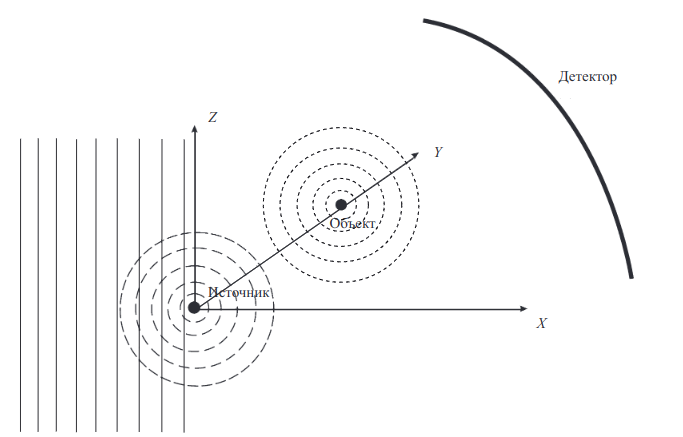
\includegraphics[scale=0.6]{ng_1}\\
Рис.16 -- Модель голографического опыта \\

Имеется первичный узконаправленный поток монокинетических нейтронов. Первый поток облучает точечный центр, некогерентно рассеивающий падающий пучок, который создает сферическую опорную волну вида: \\

$\psi_0 = \frac{e^{i\overrightarrow{k}\overrightarrow{R}}}{|\overrightarrow{R}|} $\\

Рассеивающая точка находится на расстоянии $d$ от источника опорной волны, и в результате рассеяния на этой точке создается объектная сферическая волна. Результат интерференции опорной и объектной волн регистрируются при помощи системы детекторов, расположенных на сфере фиксированного радиуса. \\

Пренебрегая затуханием опорной волны на малом расстоянии до рассеивающей точки, представим объектную волну в виде: \\

$\psi=\alpha\frac{e^{i(|\overrightarrow{k}| |\overrightarrow{d}| + |\overrightarrow{k}||(\overrightarrow{d}-\overrightarrow{R})| )}}{|\overrightarrow{d}-\overrightarrow{R}|}$ ,\\

где:\\

$\alpha$ - коэффициент, характеризующий амплитуду вторичного рассеяния, \\
$\overrightarrow{d}$ - вектор, направленный из опорного источника на объект, \\
$\overrightarrow{R}$ - вектор, направленный от источника на выбранную на детекторе точку, \\
$\overrightarrow{k}$ - волновой вектор соответствующей сферической волны. \\

Возникающая в процессе построения формы объекта проблема однозначности может быть снята путем изменения в некотором диапазоне энергии нейтронов пучка. \\

Эксперимент по рассеянию нейтронов ставится всегда так, что $R\gg d$. Неравенство это выполняется с большим запасом, так как величина d имеет порядок $10^{-10}$м, а R - порядка 1м. Детекторы располагаются так, что R = const. \\

Вероятность регистрации нейтрона $P$ в данной точке сферы описывается обычной интерференционной формулой: \\

$P=P_0(1+2\alpha(kd(1-cos\Theta ))) + O(\alpha)$ \\

где: \\

$\Theta $ - угол между направлением на детектор и направлением на объект, \\

$P_0$ - интенсивность, соответствующая "засветке" регистрирующей системы от источника в отсутствии интерференции двух рассеянных сферических волн, \\

$O(\alpha) \ll 0$ - поправки более высоких порядков малости, которыми в дальнейшем будем пренебрегать\\

Полученная формула позволяет понять причину отмеченной выше неоднозначности восстановления положения рассеивающей нейтронный поток точки: величина $d$ стоит в аргументе функции косинус, и изменение её знака не меняет структуру голограммы. \\

На следующих фотографиях приведены виды сферической голограммы для двух различных значений $d$: \\

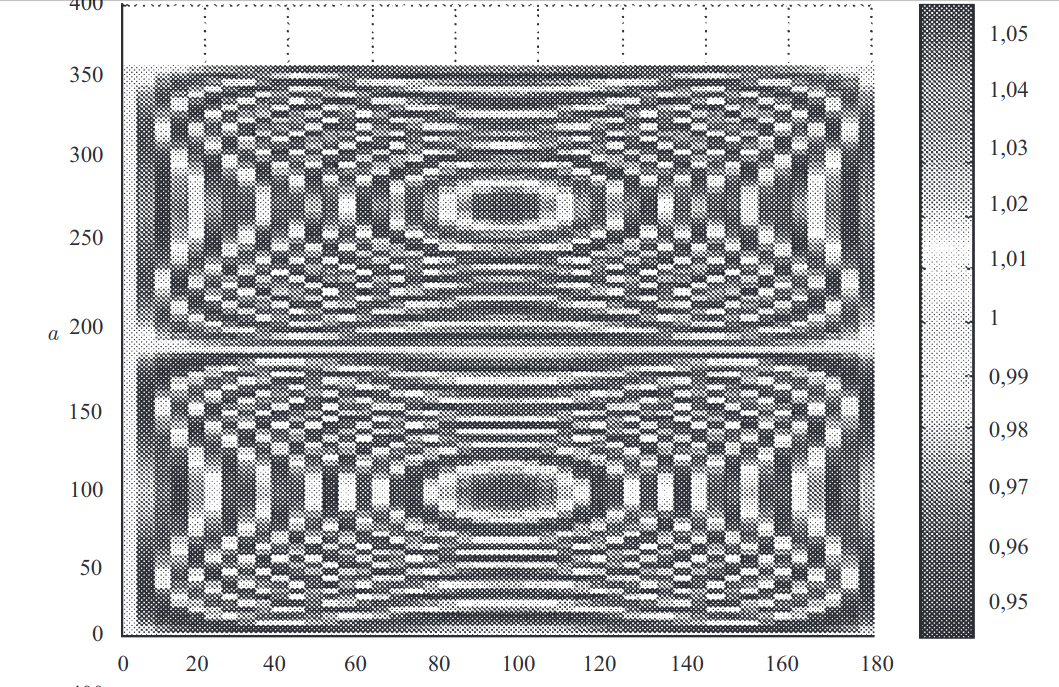
\includegraphics[scale=0.4]{ng_2}\\
Рис.17 -- $d=4\stackrel{o}A$\\

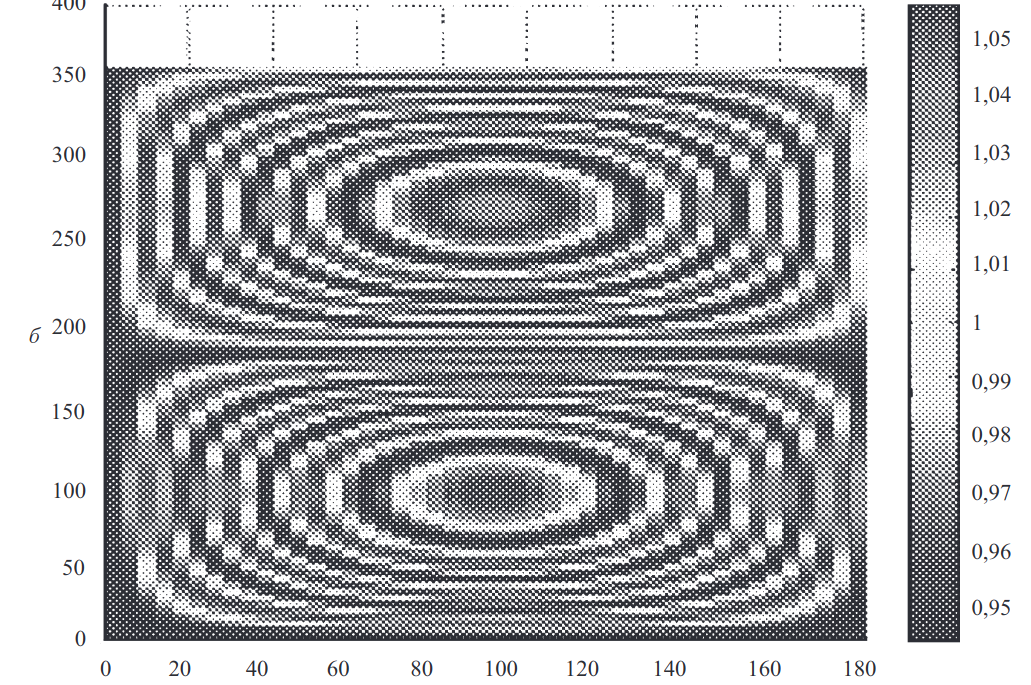
\includegraphics[scale=0.4]{ng_3}\\
Рис.18 -- $d=2,5\stackrel{o}A$\\

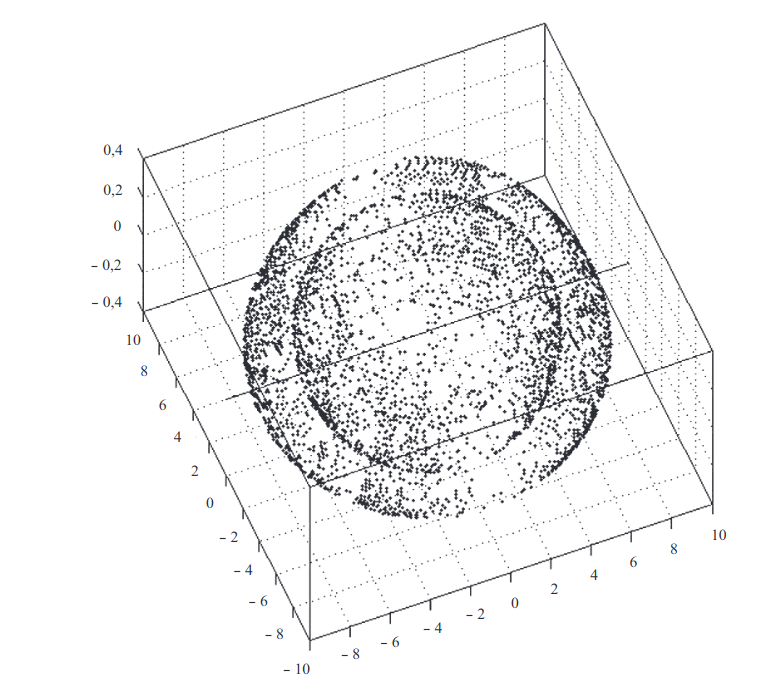
\includegraphics[scale=0.4]{ng_6}\\
Рис.19 -- Пространственное распределение вероятности для $J/J_0 = 0,1 $\\

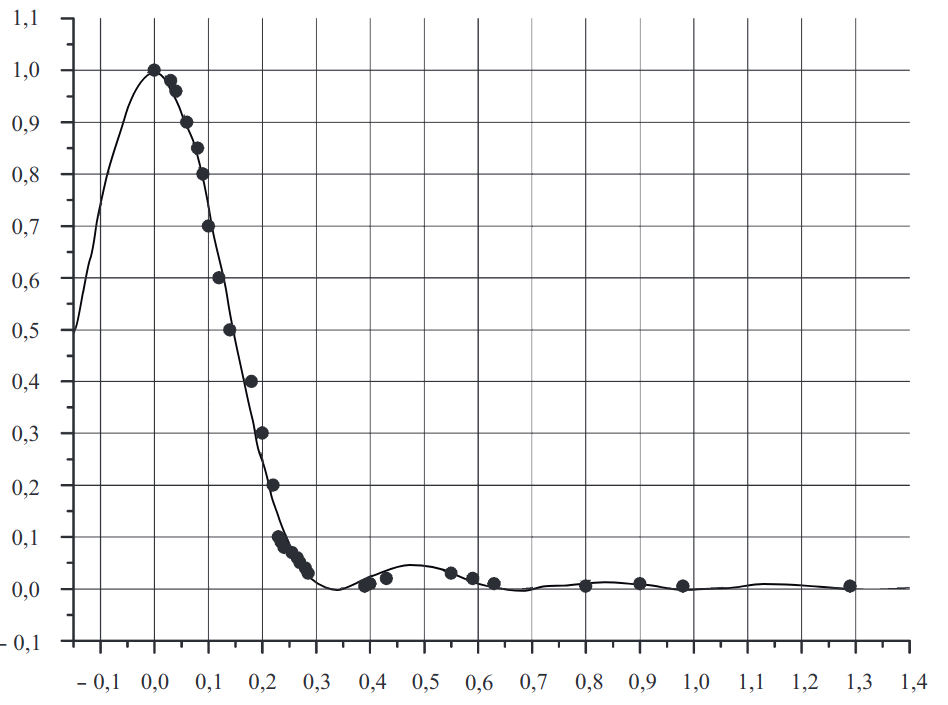
\includegraphics[scale=0.4]{ng_5}\\
Рис.20 -- Зависимость $J/J_0$  от расстояния\\

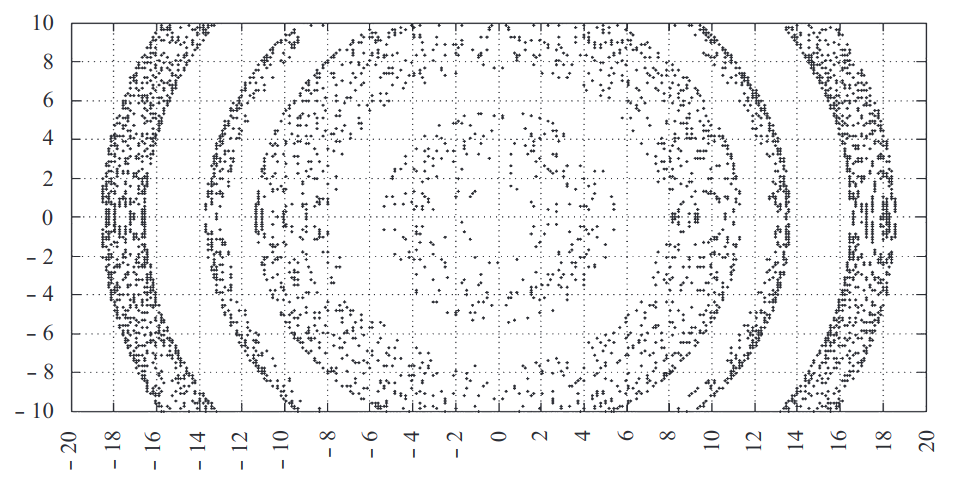
\includegraphics[scale=0.4]{ng_4}\\
Рис.21 -- Образование множества слоев при $J/J_0 = 0,005 $\\

\subsection{Отражение поляризованных нуклоноов}
Для нашего простейшего квантового компьютера кроме координат, задающих первый кубит, нужны еще и спины, задающие второй кубит. Для этого рассмотрим теорию отражения поляризованных нейтронов.


\subsection{Дифракция заряженных лучей}
При дифракционном рассеянии заряженных частиц ядрами величина $S_l$ даже при больших $l$ отлична от единицы вследствие кулоновского взаимодействия, существующего при сколь угодно больших величинах прицельных параметров. \\

Амплитуда рассеяния для $\Theta > \Theta_C$, где $\Theta_C \approx \frac{2n}{kR} \gg 1$ - критический угол до которог основной вклад в сечение дает кулоновское рассеяние, а больше которого - ядерное дифракционное рассеяние. \\

$f_n(\Theta) = ik \int_0^∞ dbbe^{2i\chi (kb)}(1-S(b))J_0(kb\Theta)$ \\

Учет поверхностного преломления приводит к появлению мнимой части матрицы рассеяния и ее интерференции с кулоновской фазой. В частности, эта интерференция приводит к различном поведению дифференциальных сечений в минимумах для упругого рассеяния частиц с противоположными знаками зарядов на одних и тех же ядрах, например $\pi^{+} $ и $\pi^{-} $ 

\subsection{Поляризация нуклонов при дифракционном рассеянии}
Так как ядерное взаимодействие зависит от спинов, то при столкновении адронов, имеющих отличные от нуля спины, может возникнуть поляризация. При рассеянии частиц со спином 1/2 ядрами с нулевыми спинами поляризация обусловлена спин-орбитальным взаимодействием. Добавляя к комплексному оптическому потенциалу спин-орбаитальный член, можно изучать на основе оптической модели поляризационные характеристики нуклонов, упруго рассеянными ядрами. 

\subsection{Заключение}
Вышеприведенное описание различных дифракционных и интерференционных картин дают теоретическое обоснование процессам во второй установке и демонстрируют разнообразие инструментов для построения квантовых операторов.

\section{Возможность визуальной видео-регистрации}
Рассчитаем требования к частоте съемки видеокамеры. Для этого определимся с интенсивностью источника. 
Пусть интенсивность калиброванного потока будет $10^3 \alpha / \text{сек} $ при энергии $E=5,3\text{МэВ} $ который рассеивается на золотой пластинах толщиной $10^{-7}$ м  (100нм) на площади датчика $ 1 cm^2 $ на расстоянии 0.1 м и углу относительно центра 10 градусов.\\

Для начала вычислим свойства: \\

Золото:\\
Плотность золота: $\rho_{Au} =1.93\cdot 10^4 $ кг/м$^3$ \\
Заряд: $Z=75$ \\
Атомная масса: $A=197а.е.м = 197 \cdot (1.66 \cdot 10^{-27}) = 3.27 \cdot 10^{-25} $ кг \\
Плотность: $\rho = \frac{1.93\cdot 10^4}{3.27 \cdot 10^{-25}} = 0.59\cdot 10^{29} $ 1/м$^3 $ \\

$\alpha$-частица \\
Заряд: $Z=2$ \\
Атомная масса: $A=4$ \\
Интенсивность: $10^3 $ 1/c \\

$ \frac{d\sigma}{d\theta}=(\frac{zZe^2}{4\pi \epsilon_02E})^2 \frac{1}{4sin^4\frac{\theta}{2}} \approx 2 \cdot 10^{-26}$ \\

$\frac{dI}{I} = \rho \delta x \frac{d\sigma}{d\omega} = 1.3 \cdot 10^{-3} $ \\

$dI = 1.3$ Гц \\

Следовательно, возможно использовать обычную видеокамеру. Современные веб-камеры снимают с частотой в диапазоне 9-90 Гц.

\chapter{Частные вопросы эскизного проектирования стендов }
\section{Стенд №1}
\subsection{Принципиальная схема}
Принципиальная схема простейшего квантового компьютера  устройства приведена на рисунке ниже:\\
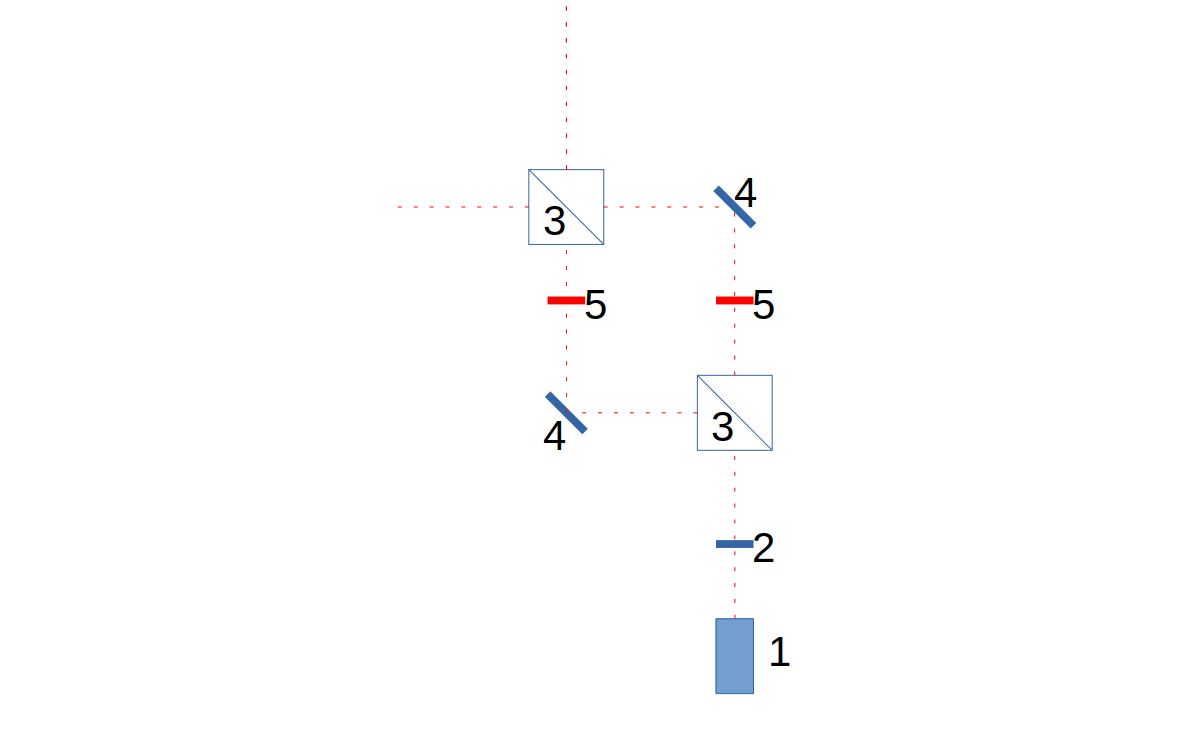
\includegraphics[scale=0.3]{ust_f} \\
Рис.22 -- Принципиальная схема стенда \\

\begin{description}
\addtolength{\itemindent}{0.80cm}
\itemsep0em 
\item[1] - лазер
\item[2] - линейный поляризатор
\item[3] - интерферометр Маха-Цендера, состоит из полупрозрачных зеркал (светоделительные кубики)
\item[4] - металлические зеркала
\item[5] - полуволновые пластины, выполняют функцию оракула 
\end{description}


\begin{figure}[h]
\center{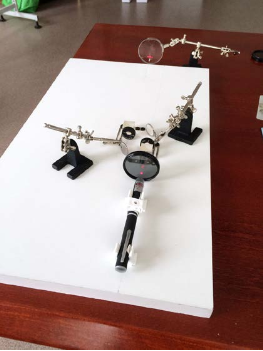
\includegraphics[scale=0.3]{ust_a_1}}
\end{figure} 

Рис.23 -- Установка в сборе  \\

\begin{figure}[h]
\center{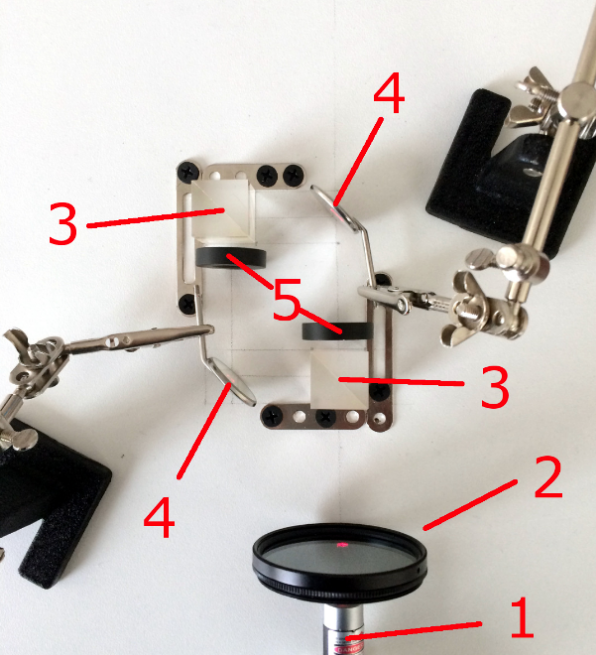
\includegraphics[scale=0.3]{ust_a_2}}
\end{figure}

Рис.24 -- более детально\\

Как видим, данная установка достаточна простая и может быть собрана на основе имеющегося оборудования лаборатории оптики. Вся сборка располагается на массивной ровной плите дсп. Лазер - источник фотонов. Длина волны не принципиальна, но необходимо, чтобы все остальные приборы соответствовали длине волны лазера. В СПБГУ в подобной установке используется красный лазер с длиной волны 650 нанометров и мощностью 100 милливат. Подобный красный лазер мощностью 50Вт стоит на AliExpress менее 1000 рублей. \\

Данная установка с изменением материалов дифракции и поляризации (кварцевые кристаллы) должна работать на холодных нейтронах, при соблюдении норм радиационной безопсаности, поэтому, для нейтронного излучения этот стенд должен быть собран внутри вакуумной камеры стенда №2, что, как договорились называть в начале, будет стендом №3 .

\subsection{Принцип действия}
Каждый фотон переносит два кубита. Первый кубит - позиция фотона в интерферометре (путь по которому проходит фотон), второй кубит - поляризация. Выйдя из лазера, фотоны проходят через линейный поляризатор. Вообще говоря, для сеанса вычисления нам достаточно одного фотона. Фотон проходит через линейный поляризатор, уже знакомый нам, и попадает в интерферометр Маха — Цендера, состоящий из двух полупрозрачных зеркал и двух обычных зеркал. Полупрозрачные зеркала выполнены в виде светоделительных кубиков. Обратите внимание, что кубики должны быть неполяризационные — они не должны менять поляризацию наших фотонов. И обычные зеркала должны быть без стеклянного покрытия, обычные металлические зеркала — поскольку стеклянное покрытие создает дополнительную отраженную волну, которая портит нам интерференцию. Такими зеркалами, например, пользуются стоматологи. Квантовый оракул у нас будет выполняться в виде вот таких вот волновых пластин, полуволновых пластин для красного цвета. Вообще говоря, волновую пластину можно простейшую сделать из куска скотча, но, для того чтобы у нас запаздывание происходило ровно на половину длины волны, надо, конечно, заказать полуволновые пластины для красного цвета. Результатом измерения для нас будет интерференционная картина: \\
\begin{figure}[h]
\center{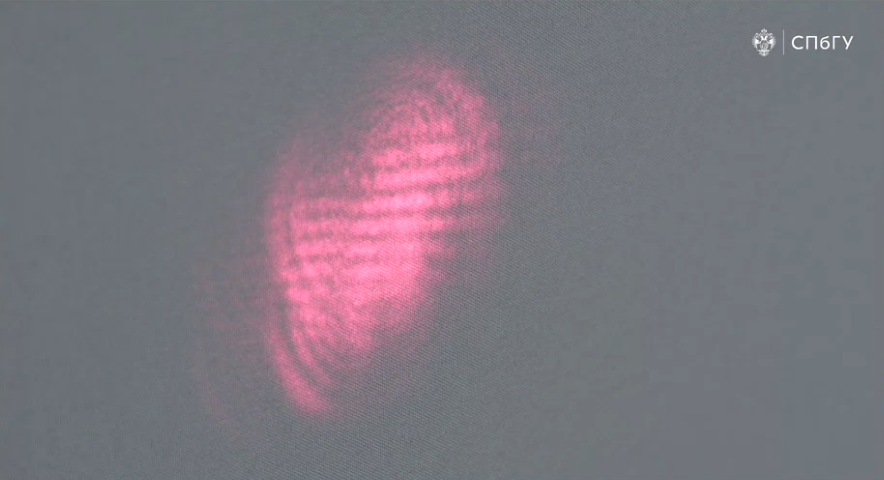
\includegraphics[scale=0.3]{inter}}
\end{figure}
Рис.25 -- Пример интерференционнной картины \\

После настройки, можно видеть результат: слева - f-сбалансирована, справа - f=const \\

\begin{figure}[h]
\center{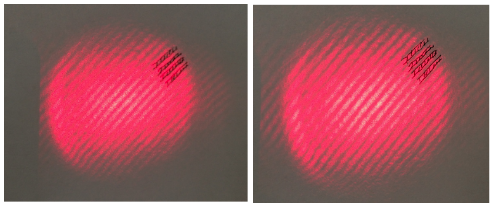
\includegraphics[scale=0.9]{inter_1}}
\end{figure}

Рис.26 -- Интерференционнной картина после настройки \\

\section{Стенд №2}
\subsection{Принципиальная схема}

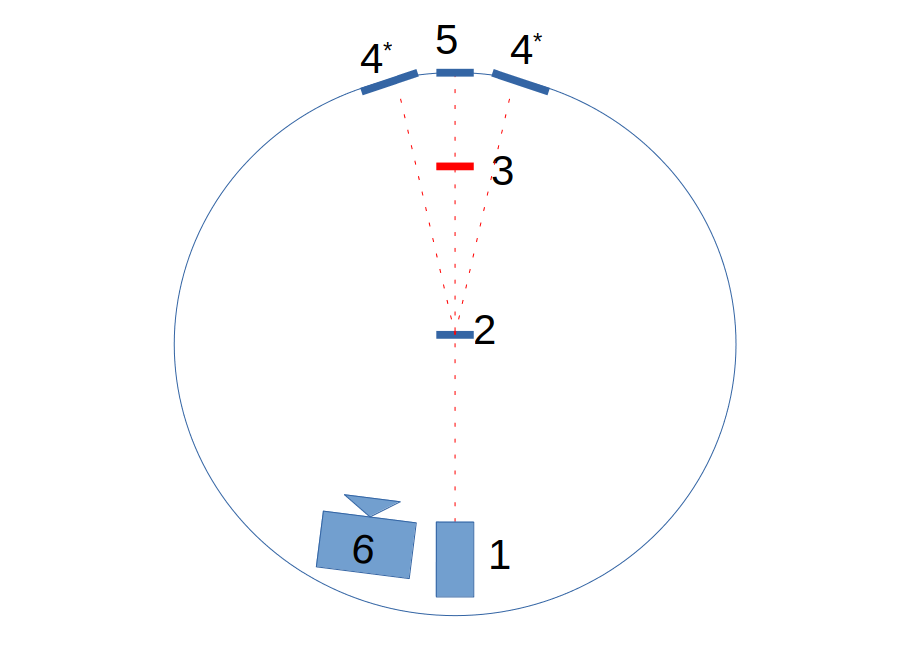
\includegraphics[scale=0.3]{ust_a}\\
Рис.27 -- Принципиальная схема стенда №2 \\

\begin{description}
\addtolength{\itemindent}{0.80cm}
\itemsep0em 
\item[1] - источник излучения
\item[2] - мишень, тонкая металлическая фольга, для эластичного рассеяния
\item[3] - мишени, сильного поглощения, выполняющие функцию оракула
\item[4] - датчики, для косвенного измерения начального потока, по известному сечению рассеяния
\item[5] - экран, пластина покрытая сульфатом цинка
\item[6] - видео камера
\end{description} 

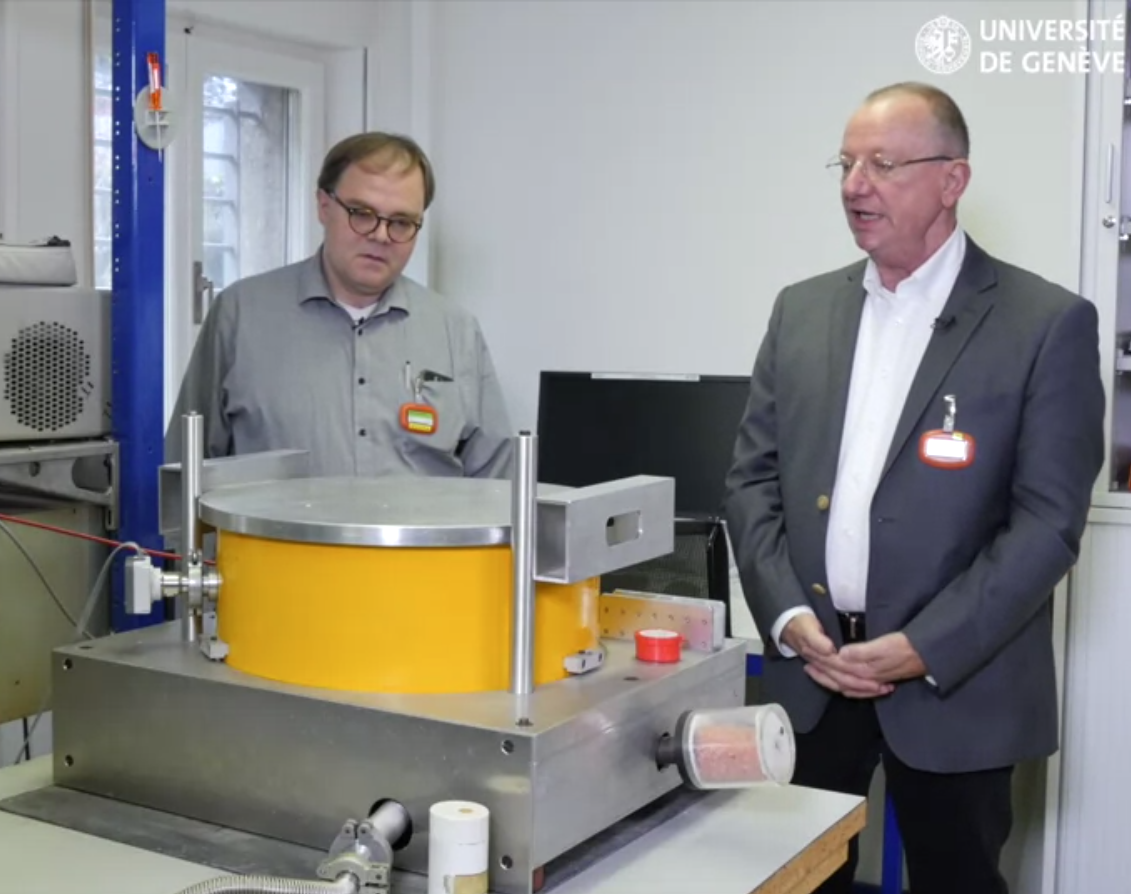
\includegraphics[scale=0.3]{ust_a_3}\\
Рис.28 -- Внешний вид стенда для проведения эксперимента Резерфорда в Женевском Университете\\

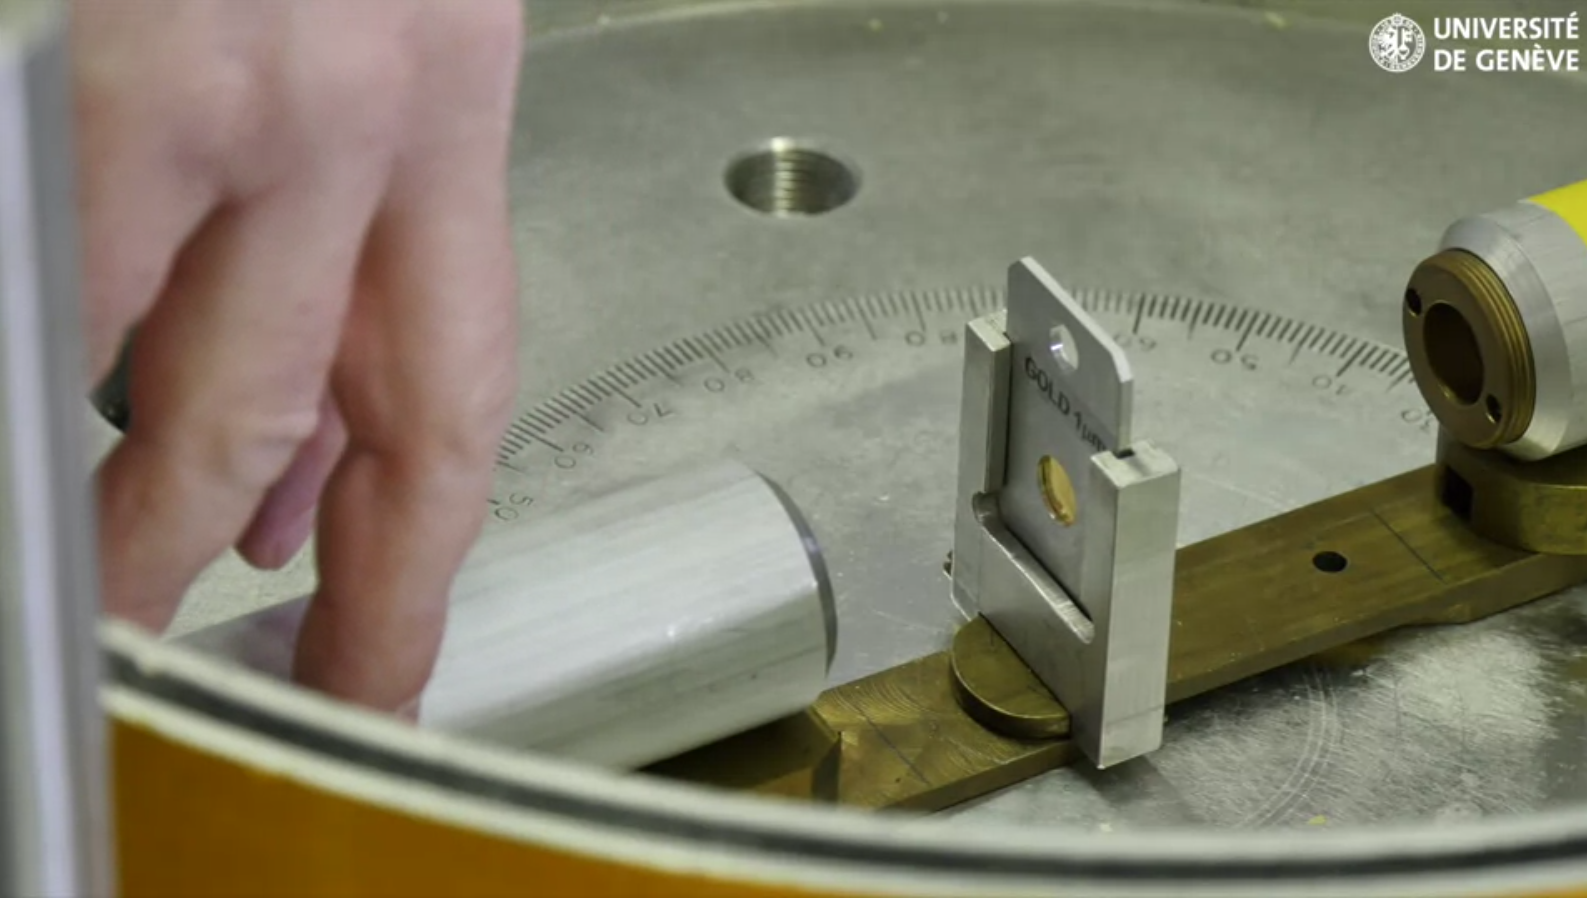
\includegraphics[scale=0.22]{ust_a_4}\\
Рис.29 -- Вид внутри вакуумной камеры\\

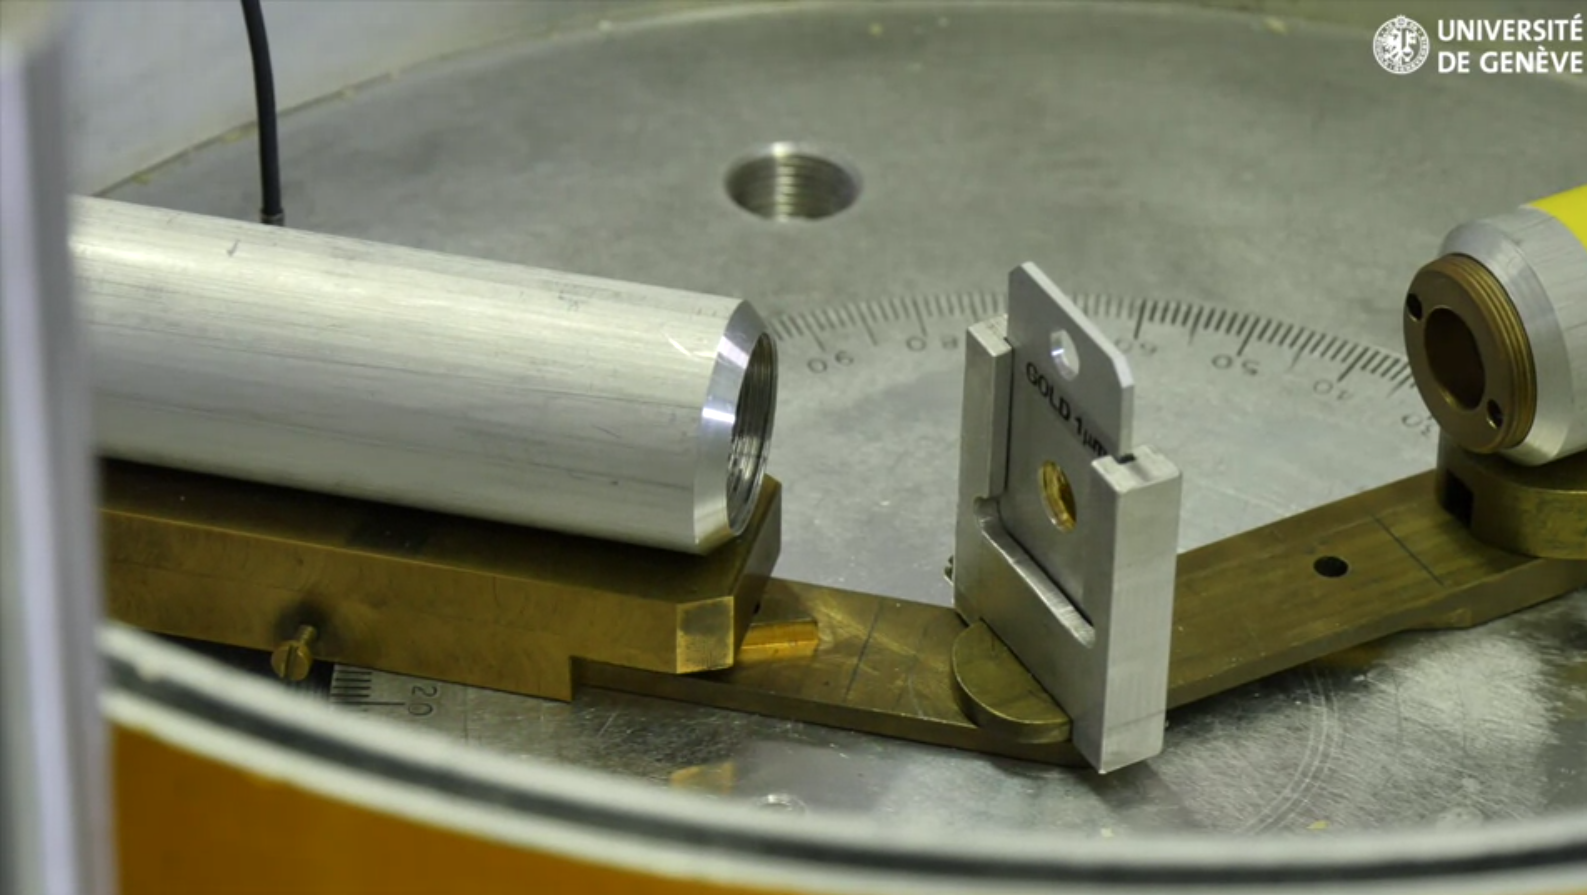
\includegraphics[scale=0.22]{ust_a_5}\\
Рис.30 -- Возможность легко изменять угол датчика - в нашем случае датчиков с изменением угла будет два\\

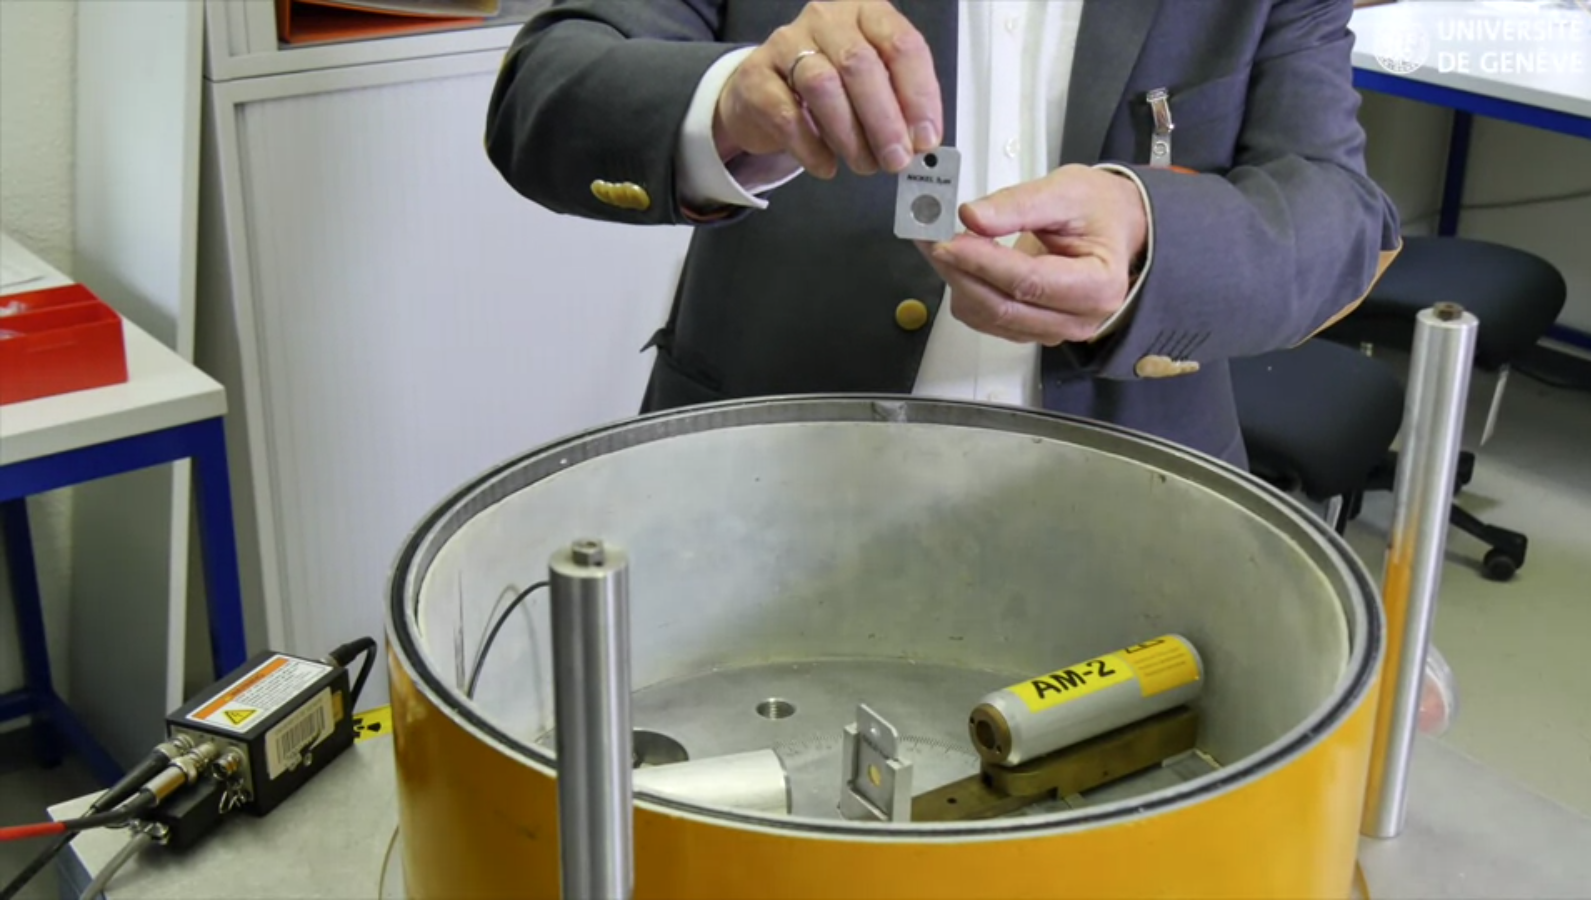
\includegraphics[scale=0.22]{ust_a_8}\\
Рис.31 -- Используются мишени различных металлов \\

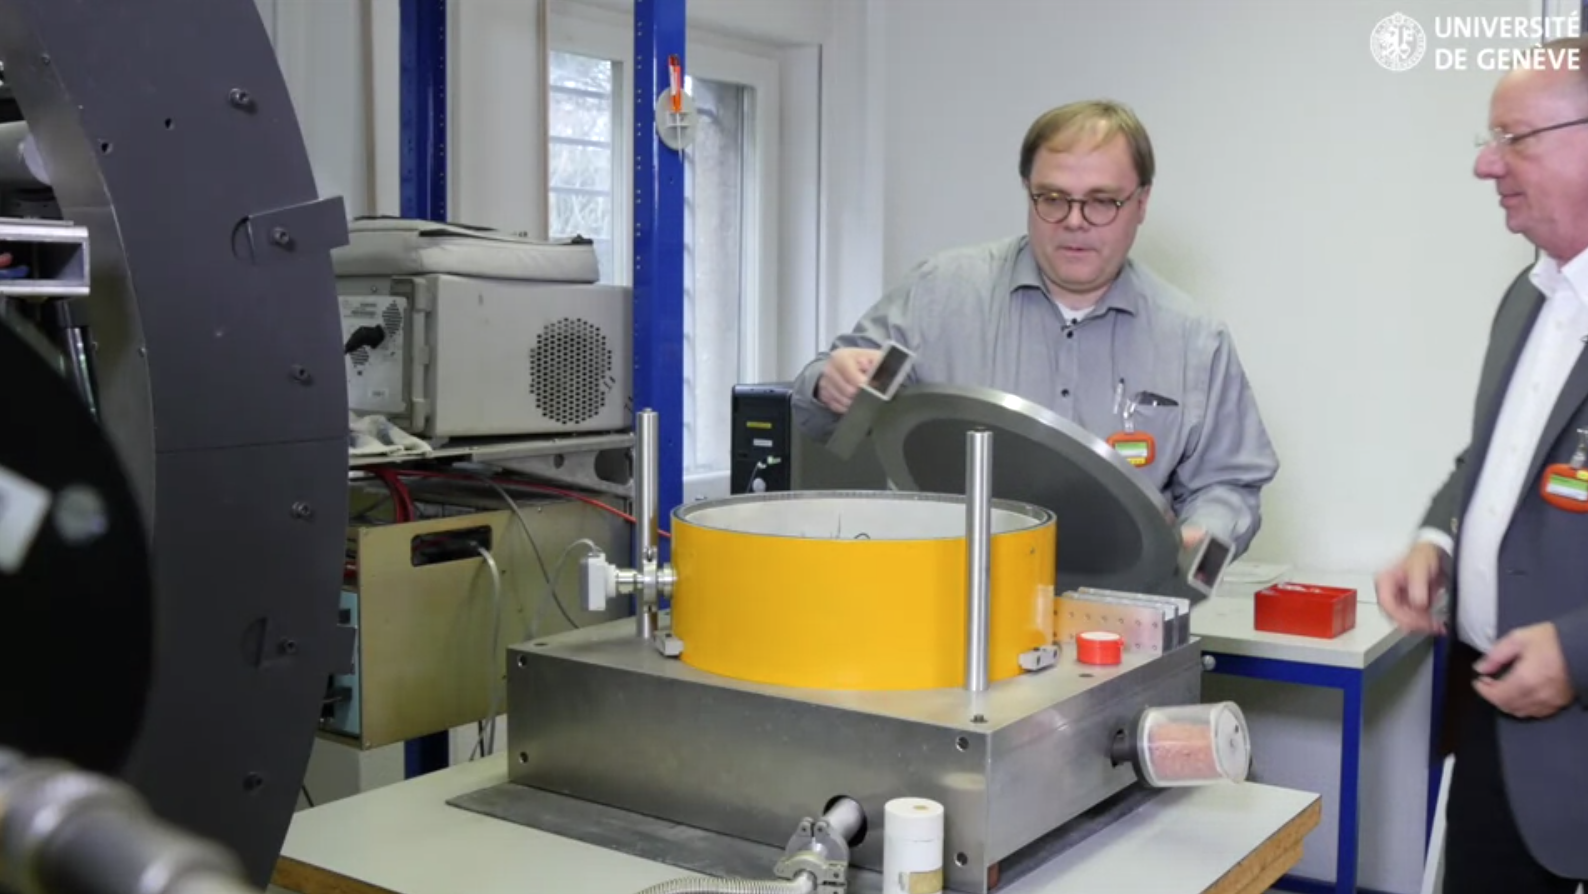
\includegraphics[scale=0.22]{ust_a_6}\\
Рис.32 -- Процесс герметизации\\

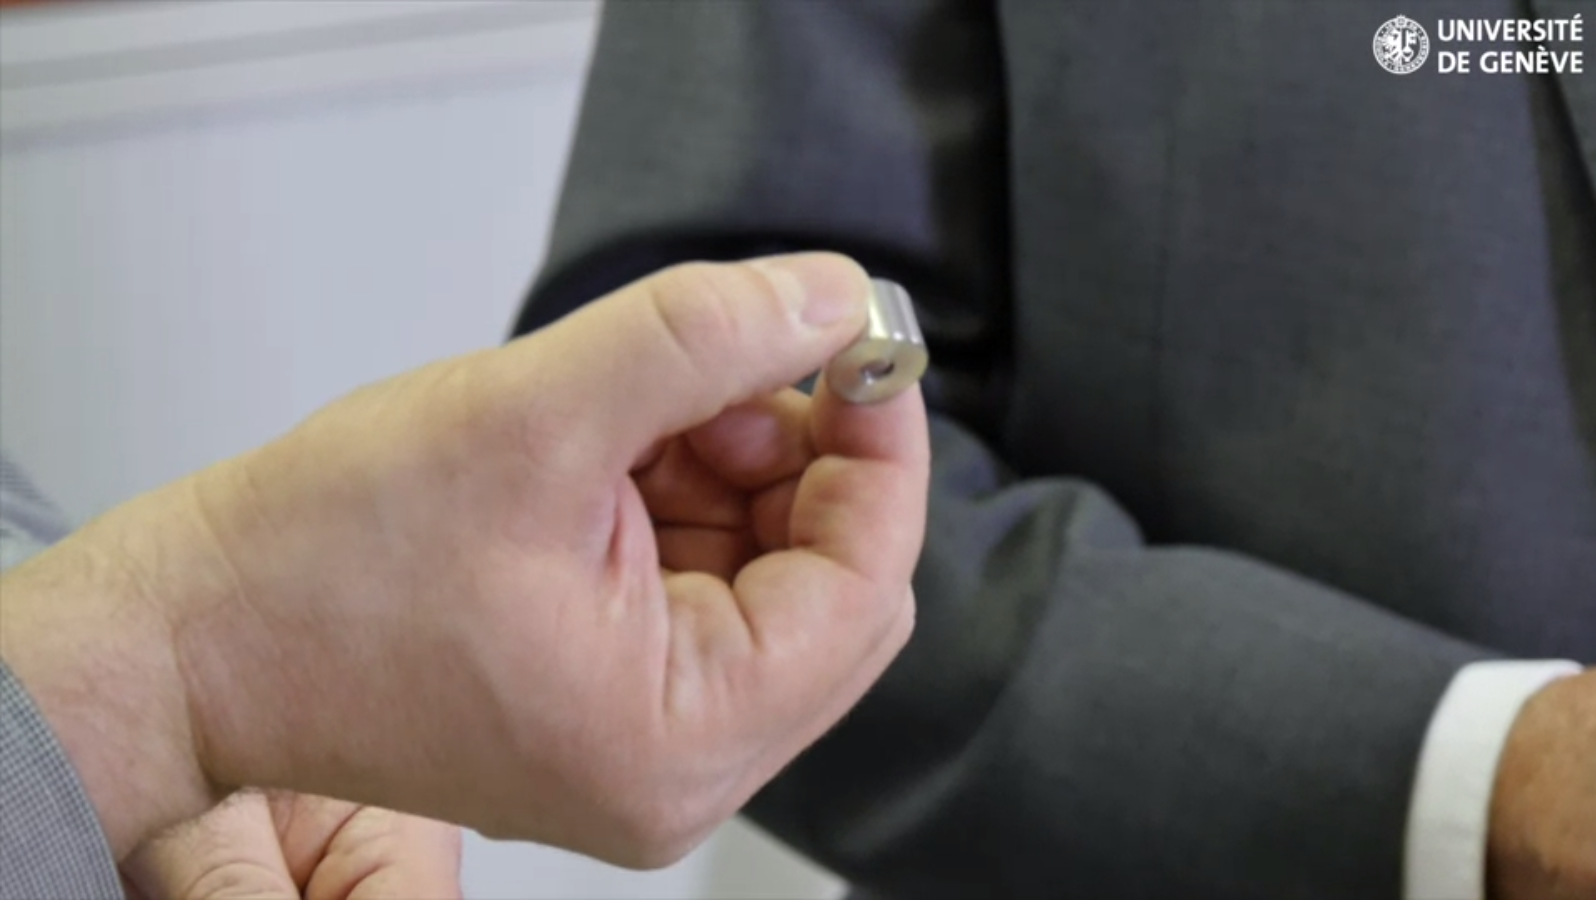
\includegraphics[scale=0.22]{ust_a_9}\\
Рис.33 -- Внешний вид используемого dE/dx кремниевого датчика:\\

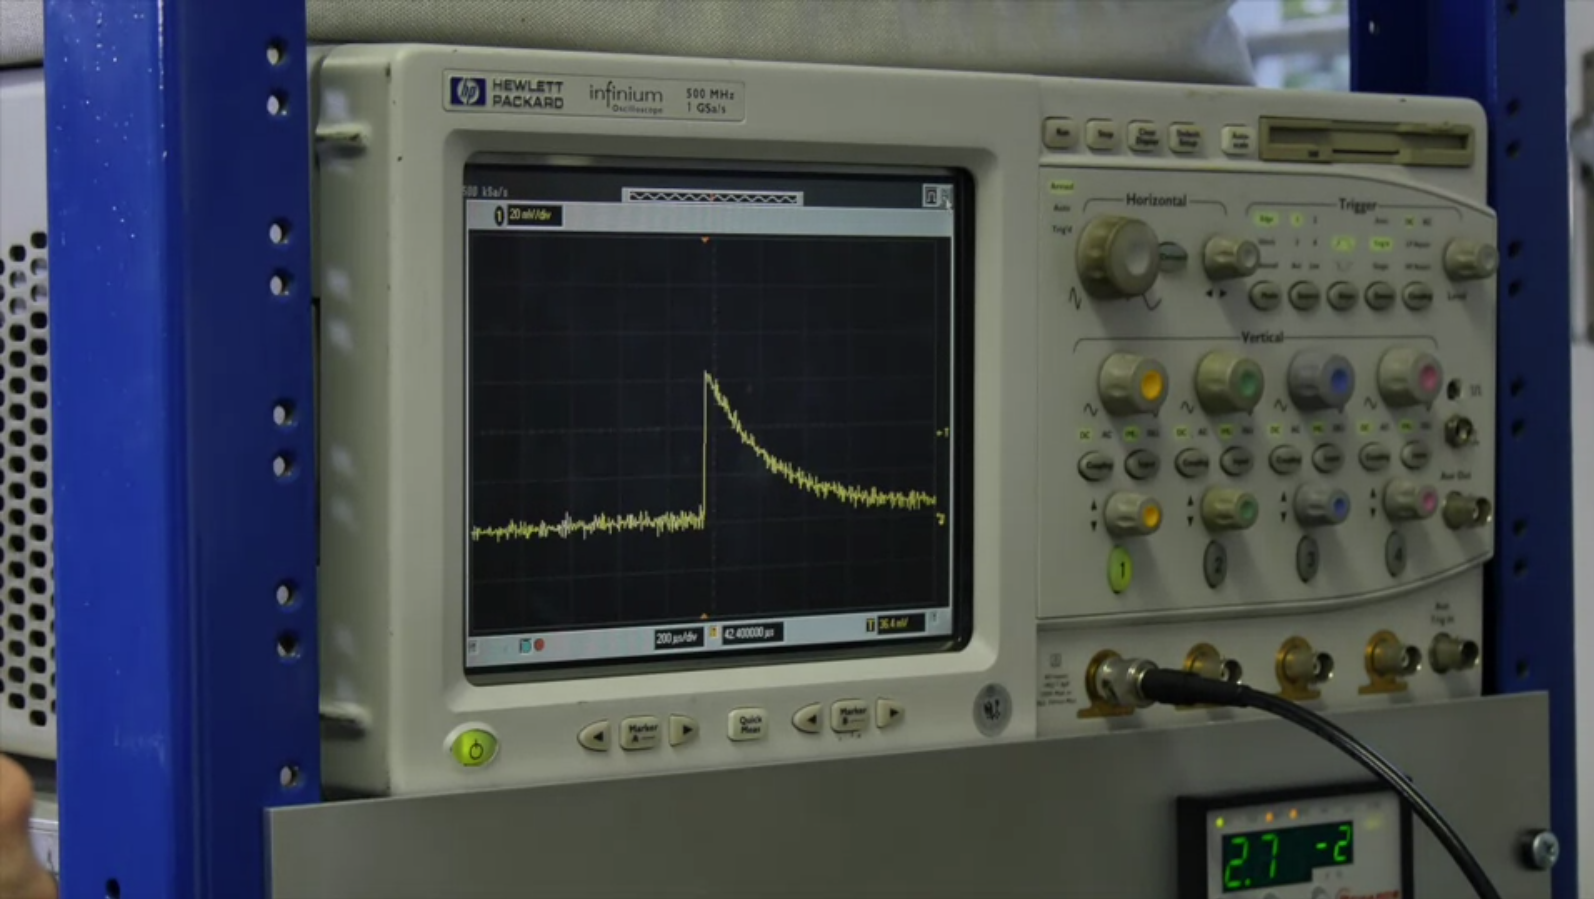
\includegraphics[scale=0.22]{ust_a_7}\\
Рис.34 -- Сигнал с датчика\\

\subsection{Принцип действия} 
Взаимодействие квантовых объектов (молекул, атомов, атомных ядер, элементарных частиц) приводят к появлению дифракционных картин, аналогичных дифракции света. Но в отличии от оптической установки, где нам приходилось создавать специальные условия для получения интерференционной картинки, в данной установке все сводится к процессам внутри материала мишени. Дифракция является общей квантово-механической картиной столкновения частиц, при условии, что одна из сталкивающихся частиц имеет конечные размеры и сильно поглощает налетающие частицы. Вопрос какой должна быть мишень и из какого материала лежит в области эксперимента. Дифракция содержится во всех моделях процессов рассеяния, как макроскопических - где мишень однородный бесструктурно поглащающий материал, так и микроскопических, в которых происходит рассеивание налетающей частицы на отдельных структурных составляющих рассеивателя.\\

Атомные ядра в довольно широкой области энергий сильно поглощают налетающие на них частицы, т.е. ведут себя как непрозрачные поглощающие экраны, поэтому, ожидается что будет наблюдаться дифракция, что требуется продемонстрировать на стенде. Есть опасения, что $\alpha$ частицы достаточно большие для атомного ядра и слишком низкоэнергетичны для появления дифракционных эффектов, что требуется проверить, однако на источнике, излучающем адроны, появление дифракции не вызывает сомнений, что, конечно, также предстоит экспериментально проверить. \\

С возрастанием энергии налетающих частиц длина их свободного пробега в ядерном веществе может оказаться сравнимой с линейным размером ядра, что приведет к снижению поглощения частиц, ядра станут полупрозрачными. Следующий фактор ухудшающий дифракцию - отсутствие четких границ у ядра, так как плотность ядерной материи постепенно уменьшается в поверхностной области ядра. Два этих параметра - прозрачность и размытие границы ядра основные параметры получаемой дифракционной картины, которыми можно варьировать, выбирая различные материалы мишени, частицы, энергии. \\

Кроме дифракционного рассеяния, наблюдается еще один аналог оптического явления - радужное сияние, которое характеризуется затуханием осцилляций дифференциального сечения и наличием широкого максимума - радужный максимум. Ядерная радуга наблюдается в основном при рассеянии легких ядер $^3$He,$^4$He, $^6$Li при энергиях $E\gtrsim 25-30$МэВ средними и тяжелыми ядрами. \\

С помощью дифракционной теории ядерного взаимодействия возможно описать зарядово-обменные реакции, расщепление сложных частиц, реакции передачи нуклонов и прочие ядерные реакции, что делает ядерную дифракцию более привлекательной для построения квантового компьютера, чем оптическая. Теоретические и экспериментальные данные дифракционной теории позволяют минимизировать квантовые системы до атомарных толщин и строить квантовые системы на базе знаний о ядерной структуре и механизмах разных ядерных процессов.

Аналогично первой установки каждая частица переносит два кубита. Первый кубит - отклонение частицы в мишене (интерферометре) (путь по которому проходит частица), второй кубит - либо поляризация, либо энергия - здесь индивидуально для каждого опыта. В материале мишене происходит дифракционное рассеяние, после чего чатицы попадают на экран с люминофором и видеокамера фиксирует вспышку. Как мы видим, данная установка более универсальна, в отличии от первой, которая работает только на фотонах.

\subsection{Требования к источникам}
В зависимости от конструкционной особенности и активности источника мишень 2 можно убрать. Также некоторые конструкции источников помогают регулировать интенсивность излучения, что кроме удобства позволит снизить требования к частоте съемки видеокамеры и качеству экрана. \\

Из предыдущего раздела, мы можем предъявить требование к источнику $\alpha$-частиц по энергии: $E\gtrsim 25-30$МэВ по активности 1000Бк. Также для нейтронного излучения: холодные нейтроны: $E_n=0.07$эВ и источник гамма квантов или фотонов $E_\gamma=12$МэВ. \\

Далее рассмотрим источники предлагаемые на сайте isotop.ru

\subsection{Источники $\alpha$ - излучения}

\begin{tabular}{|p{2.5cm}|p{2.7cm}|p{2.5cm}|p{1.5cm}|p{5cm}|}
\hline
	Элемент & Тип/код источника & $I_{\alpha}$, Бк & $E_{\alpha}$, МэВ & Назначение\\
\hline
	Америций-241 & АРИА(обр) \linebreak AAm1.1.S1 \linebreak AAm1.1.S2 \linebreak AAm1.2.S1 & - \linebreak 500 \linebreak 1000 \linebreak 3000 & $5,4-5,5$ & Эталонные и контрольные источники\\
\hline
	Кюрий-244 & АЗК244.28 & $\geq 1,4\cdot 10^8$ & $\leq 5,2 $ & Для рентгенофлюоресцентного анализа\\
\hline
	Плутоний-239 & АИП-МИР-3А \linebreak АИП-РИГ \linebreak АДИ \linebreak АИП-РИД \linebreak АИП-ЭДГХ & 5,9$ \cdot 10^7$ \linebreak 4,10$\cdot 10^7$ \linebreak 2,1$\cdot 10^7$ \linebreak 2,1$\cdot 10^5$ \linebreak 2,1$\cdot 10^7$ \linebreak & $\leq 5,2 $ & извещатели дыма, газовая хромотография, газоанализаторы, герметичные - придется разбирать\\
\hline
	Pu-239\linebreak \linebreak \linebreak  U-234 \linebreak \linebreak \linebreak U-238 \linebreak & 1П9 2П9 3П9 4П9 5П9 6П9 \linebreak \linebreak 1У4 2У4 3У4 4У4 5У4 6У4 \linebreak \linebreak 1У8 2У8 3У8 4У8 5У8 6У8 \linebreak & 4-1,6$\cdot 10^7$ \linebreak \linebreak \linebreak 1$\cdot 10^1$ - 1$\cdot 10^3$ & $\leq $5,2 \linebreak \linebreak \linebreak $\leq $4,8 \linebreak \linebreak \linebreak $\leq $4,3 & для проверки и градуировки радиометрической аппаратуры в качестве мер активности\\
\hline
\end{tabular}

Из приведенных в таблице данных можно сделать вывод, что оптимальным будет использование датчика AAm1.1.S2, а также то, что источника с энергией достаточной для появления радужного сияния нет, поэтому это будет являться ограничением данной установки.

\subsection{Источники нейтронов}
\begin{tabular}{|p{3.5cm}|p{2.7cm}|p{2cm}|p{1.5cm}|p{4.5cm}|}
\hline
	Элемент & Тип/код источника & $I_n$, Бк & $E_n$, МэВ & Назначение\\
\hline
	$^{252}$Cf \linebreak Калифорний-252 & NCf2.P01 & 1200-40000 & 2,12 & источник нейтронного излучения \\
\hline
	$^{244}$Cm \linebreak Кюрий-244 & NCm4.15.1 NCm4.15.2 NCm4.15.3 NCm4.15.4 & $0,1\cdot 10^4 - 3,0\cdot 10^4$ & быстрые & источник нейтронного излучения \\
\hline
	$^{244}$Cm \linebreak Кюрий-248 & НК248М11.44 НК248М11.26  & $\leq 2,3\cdot 10^5$ & - & источники нейтронного излучения закрытые используются в качестве образцовых при аттестации источников нейтронного излучения и и установок для нейтронных измерений.\\
\hline
\end{tabular}
Из приведенных в таблице источников наиболее подходящим видится НК248М11.44 как источник низкоэнергетических нейтронов.

\subsection{Источники $\gamma$-излучения}
\begin{tabular}{|p{2.5cm}|p{2.7cm}|p{2cm}|p{2.5cm}|p{4.5cm}|}
\hline
	Элемент & Тип/код источника & $I_{\gamma}$, МБк & $E_{\gamma}$, МэВ & Назначение\\
\hline
	$^{238}$Pu+$^{13}$C  & GPu8-C3 & $\leq$0,185 & 6,13 & эталонный источник \\
\hline
	Кобальт-57 \linebreak Кобальт-60 \linebreak Барий-133 \linebreak Цезий-137 & ОИДК & 0,037-370 \linebreak 0,037-3,7 \linebreak 0,037-37 \linebreak 0,037-37 & 0,0144 - 0,1365 \linebreak 1,1732 - 1,3325 \linebreak 0,0810-0,38385 \linebreak 0,6617 & эталонный источник \\
\hline
	Натрий-22 \linebreak Титан-44 \linebreak Марганец-54 \linebreak Железо-55 \linebreak Кобальт-57 \linebreak Кобальт-60 \linebreak Цинк-65 \linebreak Иттрий-88 \linebreak Кадмий-109 \linebreak Олово-113 \linebreak Барий-133  & ОСГИ & 0,001-1,000 & 1,274 \linebreak 0,0689-1,157 \linebreak 0,8348 \linebreak 0,0059-0,0065 \linebreak 0,0144-0,1365 \linebreak 1,1732-13325 \linebreak 1,11554 \linebreak 0,898-1,8361 \linebreak 0,088 \linebreak 0,2551-0,3917 \linebreak 0,081-0,356 & для проверки и градуировки средств измерений фотонного излучения \\
\hline
\end{tabular}

Анализируя данные таблицы интересным представляются источники ОСГИ для проверки фотонных детекторов. Возможно заменить лазер в оптической установке данным источником, если это удешевит установку, либо сделать этот стендуниверсальным - совместить с оптическим стендом.

\subsection{Источники $\beta$-излучения}
\begin{tabular}{|p{3.5cm}|p{2.0cm}|p{2cm}|p{2.5cm}|p{4.5cm}|}
\hline
	Элемент & Тип/код источника& $I_{\beta}$, МБк & $E_{\beta}$, кэВ & Назначение\\
\hline
- \linebreak Углерод-14 \linebreak Кобальт-60 \linebreak Никель-63 \linebreak \linebreak Стронций-90+\linebreak Иттрий-90 \linebreak \linebreak Рутений-106+Родий-106 \linebreak\linebreak Цезий-137 \linebreak Прометий-147 \linebreak Таллий-204 & ОРИБИ &  1$\cdot 10^2$-1$\cdot 10^4$ & - \linebreak 49,44 \linebreak 96,9 \linebreak 17,1 \linebreak \linebreak 196,3  \linebreak 928 \linebreak \linebreak 96,9 \linebreak \linebreak \linebreak 179 \linebreak 62,1 \linebreak 238,3 & Набор ОРИБИ предназначен для градуировки и поверки радиометров и радиометрических установок, а также для поверки зависимости чувствительности радиометров от энергии внешнего бета излучения \\
\hline
\end{tabular}
Для лучшего детектирования видится целесообразным использование высокоэнергетичных частиц, с источником на Иттрий-90


\subsection{Датчики}
Датчики можно использовать как промышленные, так и самодельные. Видится возможным создание сплошного монитора нейтронного излучения на секторе стенки вакуумной камеры на основе Лаймановского альфа-излучения. \\

В качестве датчиков счета частиц предлагается, в качестве примера, рассмотреть продукцию ООО "Западприбор", зарегистрированного в г.Москва. Сведем данные по ним в таблицу:\\
\begin{tabular}{|p{2.5cm}|p{3.5cm}|p{8.5cm}|}
\hline
	Тип & Код & Назначение\\
\hline
	Поверхностно-барьерные детекторы  & ДКПс-25 \linebreak ДКПс-35 \linebreak ДКПс-50 \linebreak ДКПс-100 \linebreak ДКПс-200 \linebreak ДКПс-350 \linebreak ДКПс-500 & спектроскопия и регистрация короткобежных заряженных частиц. Используются в лабораторных экспериментах. Залиты эпоксидной смолой.\\
\hline
	Поверхностно-барьерные кремниевые детекторы  & ДКПсд-20 \linebreak ДКПсд-50 \linebreak ДКПсд-125 & спектроскопия и регистрация короткобежных заряженных частиц. Используются в лабораторных экспериментах. Реагируют на свет. Требуют защиты. Требуют вакуум $10^{-5}$-$10^{-1}$ мм рт.ст.\\
\hline
	Детекторы кремниевые поверхностно-барьерные полностью обедненные & ДКПО-dE/dx-25 \linebreak ДКПО-dE/dx-50 \linebreak ДКПО-dE/dx-125 \linebreak ДКПО-dE/dx-200 & Широко используются для создания ядерных "телескопов", а также для измерения удельных ионизационных потерь dE/dx регистрируемых частиц.\\
\hline
	Детекторы кремниевые диффузионно-дрейфовые & ДКДПс-25 \linebreak ДКДПс-50 \linebreak ДКДПс-100 \linebreak ДКДПс-125 \linebreak ДКДПс-200 \linebreak ДКДПс-250 \linebreak ДКДПс-350 \linebreak ДКДПс-500 & можно использовать в приборах автоматического контроля процессов с применением бета-активных препаратов для измерения плотности потока электронов.\\
\hline
	Диффузионно-дрейфовые детекторы матричного типа & МДКД-П-10 \linebreak МДКД-П-20 \linebreak МДКД-П-30 \linebreak МДКД-П-40 & эффективны для определения загрязненности воздуха, поверхностей рук и других предметов радиоактивными нуклидами, изучающими альфа- и бета-частицы.\\
\hline
	Диффузионно-дрейфовые полностью обедненные детекторы & ДКПО-Д-0,5-50 ДКПО-Д-1,0-50 ДКПО-Д-1,5-50 ДКПО-Д-2,0-50 ДКПО-Д-0,5-100 ДКПО-Д-1,0-100 ДКПО-Д-2,0-100 ДКПО-Д-0,5-200 ДКПО-Д-1,0-200 ДКПО-Д-2,0-200 & могут работать при давлении ниже 10$^{-1}$ мм.рт.ст. Конструктивно несколько отличаются от ДКПО-de/dx, однако одинаковые внешние диаметры корпусов указанных типов позволяют использовать их вместе для сборки в "телескопы".\\
\hline
\end{tabular}

Для альфа излучения: датчики аналогичные ДКПО-dE/dx используются в экспериментальной установке в Университете Женевы. В процессе экспериментов нужно будет понять стоит ли собирать "телескопы" и разницу между ДКПО-Д-0,5-50 и ДКПО-dE/dx-25 датчиками. \\

Для альфа- и бета- чатиц: Д1А\\

Для нейтронного и гамма- излучения излучения: СППД1 \\

Поскольку датчики выбраны в качестве примера и авторы не настаивают на их примененит, ниже приводятся характеристики для поиска аналогов:\\

ДКПО-Д-0,5-50 \\
  Описание:детектор кремниевый диффузионно-дрейфовый полностью обедненный по диффузионно-дрейфовой технологии:\\
Площадь чувствительной области, S=50мм$^2$ \\
Энергетическое разрешение $\eta$ не более 35кэВ (для $E_\alpha $=5,15МэВ $ ^239 $Pu) \\
Рабочее напрядение 10-100В \\
Толщина чувствительной области W = 0,3-0,5мм \\
Обратный ток $I_{o}$ не более 3 мкА \\
Габаритные размеры (без выводов) d=8; D30x50 \\


ДКПО-dE/dx-25\\
Описание: прострельный детектор, у которого обедненная область простирается на всю толщину полупроводникового материала, то есть от переднего до заднего контакта. Входным окном служит с одной стороны пленка золота толщиной 12-20мкм, с другой - пленка алюминия толщиной 40-60нм. Потери в мертвом слое входного окна составляют 8-10кэВ. Рабочее напряжение 10-150В. Детекторы могут работать при давлении ниже $10^-2$мм.рт.ст.и температуре окружающей среды 0т -50 до 0 градусов цельсия или при давлении 2 кгс/см$^2$ и ниже при температуре от 0 до +50 градусов. \\
Площадь чувствительной области, S=30мм$^2$ \\
Энергетический эквивалент шума $Q$ не более 20кэВ\\
Толщина чувствительной области А W = 20-30мкм \\
Толщина чувствительной области Б W = 30-50мкм \\
Толщина чувствительной области В W = 50-80мкм \\
Толщина чувствительной области Г W = 80-130мкм \\
Толщина чувствительной области Д W = 130-200мкм \\
Обратный ток $I_{o}$ не более 3 мкА \\
Габаритные размеры (без выводов) d=5,6; D30x5 \\

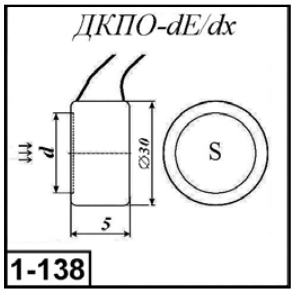
\includegraphics[scale=0.4]{dkpo_de_dx} \\
Рис.36 - внешний вид детекторов  ДКПО-Д-0,5-50, ДКПО-dE/dx-25\\

Д1А\\
Описание: обратно-смещенные диоды из монокристаллического кремния, изготовленные по технологии ионной имплантации. Регистрируемое излучение альфа-, бета-частицы, осколки деления и т.п.\\
Площадь чувствительной области, S=100мм$^2$ \\
Размер входного окна 10x10мм \\
Толщина чувствительной области W = 100-350мкм \\
Толщина мертвого слоя 4000А
Энергетическое разрешение для альфа-излучения с энергией 5,5МэВ при оптимальном напряжении смещения 18кэВ \\

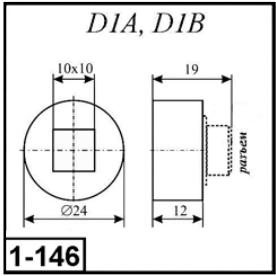
\includegraphics[scale=0.4]{d1a} \\
Рис.37 - внешний вид детектора Д1А\\

СППД1\\
Описание: полупроводниковый кремниевый детектор нейтронного и гамма-излучения, предназначен для преобразования импульсных потоков гамма-квантов и нейтронного излучения при работе в динамическом режиме в электрический аналог и могут быть использованы в различных системах регистрации. \\
Чувствительность к $\gamma$-излучению, $^{60}$Co $(0,8-2,5)\cdot 10^{-16}$ Кл $\cdot $ см$^2 $\\
Чувствительность к нейтронам, 14Мэв $(0,7-2,4)\cdot 10^{-15}$ Кл $\cdot $ см$^2 $ \\
Временное разрешение 6нс \\
Сопротивление нагрузки 75 Ом\\
Выходной линейный ток не менее 20А\\
Напряжение питания 1800$\pm$20 В \\

\subsection{Усилитель сигнала}
Усиление сигнала с датчика осуществляется двумя операционными усилителями и оцифровывается на базе Arduino c дальнейшей передачей сигнала в компьютер по USB интерфейсу. \\

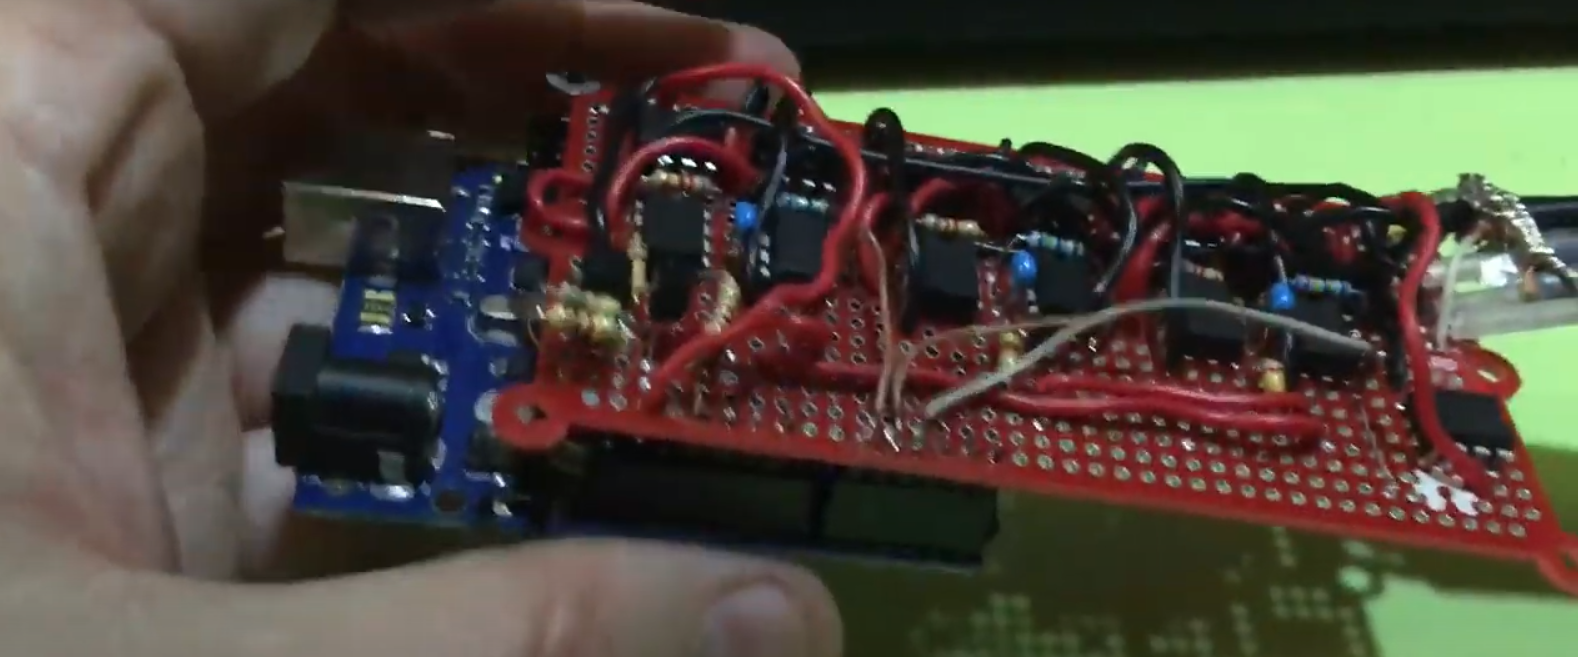
\includegraphics[scale=0.18]{ust_f_1}\\
Рис.38 - внешний вид усилителя сигнала \\

Выбор операционные усилителей не принципиален. Хорошо зарекомендовали себя в работе усилители фиры Analog Devices. AD620 имеет широкий диапазон напряжения питания (2,3В-18В), что позволит использовать в одной цепи питания вместе с датчиками (10-100В). \\


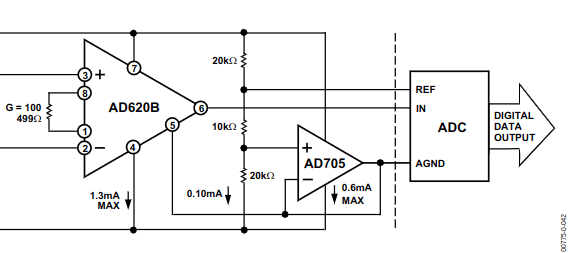
\includegraphics[scale=0.6]{ad_620}\\
Рис.39 -- Принципиальная схема усилителя\\

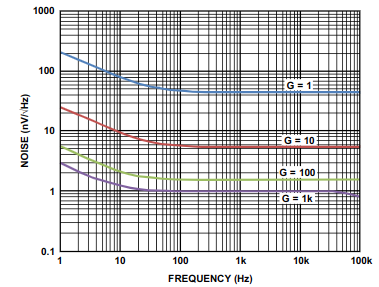
\includegraphics[scale=0.8]{ad_8249}\\
Рис.40 -- Улучшенная по снижению шума является AD8429BRZ

\subsection{Эскиз}
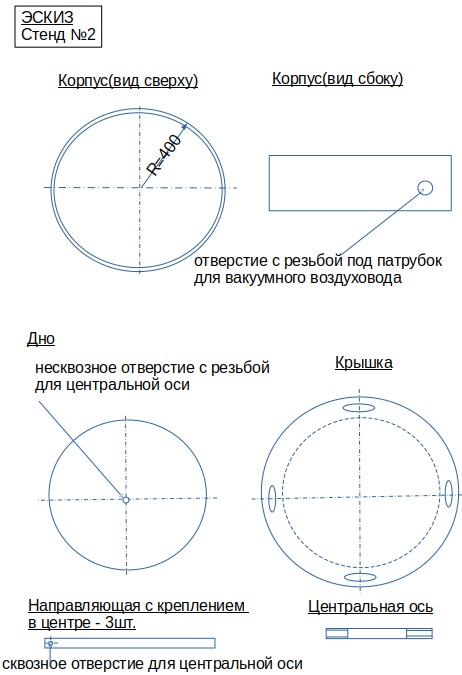
\includegraphics[scale=0.8]{stend_2}\\
Рис.41 - Эскиз Стенда №2 \\

\section{Стенд №3 }
У рассмотренных двух стендов есть свои преимущества, свои недостатки. Попробуем объеденить два стенда вместе. Т.е. вычисления вести на фотонах, а фотоны получать из частиц ядерного реактора. Для этого соберем оптическую установку внутри вакуумной камеры второй установки, только лазер заменим собственным генератором фотонов. \\

\subsection{$\alpha$-излучение Лаймана} 
Обнаружение $\alpha$-излучение Лаймана было опубликовано в ~\cite{Lymon_1} - это свет с длинной волны 121,6 нм, возникающий при переходе с $n=2$ в $n=1$ в атомарном водороде, как продукт ядерной реакции $^3 $He(n,tp) происходящей в ячейке с газом $^3 $He.\\

$^3 $He + $n \rightarrow ^3$ H $^{+}$ + $^1 $H$^{+}$+ 764 кэВ\\

Экспериментальные результаты по изучению это реакции были опубликованы в ~\cite{Lymon_2}. Было подсчитано, что на каждый медленный нейтрон ($\lambda_n=$0,496 нм ), поглощенный в разряженной до 93кПа камере , содержащей $^3 $He производилось 46 Лаймовских альфа-фотонов $\gamma_\alpha$.\\

Такое количество связано с процессом "перезарядки" чатиц, когда электрон частицы переходит на возбужденную орбиталь, затем испускается фотон, электрон переходит на более низкую и так далее.\\

Были вычислены доли процессов, в образовании $\gamma_\alpha$-излучения, а именно: столкновения $^3 $H$^{+}$ (тритоны), $^3 $H$^{+}$, $^1 $H$^{+}$(протоны), $^3 $H(тритий), $^1 $H(атомы водорода) с фоновым газом $^3 He$ в камере, а также пространственное распределение производимого излучения.\\

Ниже приведены два примера процесса:\\

p+He $ \rightarrow $H(2p)+He$ ^{+} \rightarrow $ H(1s)+$\gamma_\alpha$ - для заряженных частиц\\

H+He$ \rightarrow $H(2p)+He$ \rightarrow $H(1s)+$\gamma_\alpha$ - для нейтральных частиц.\\

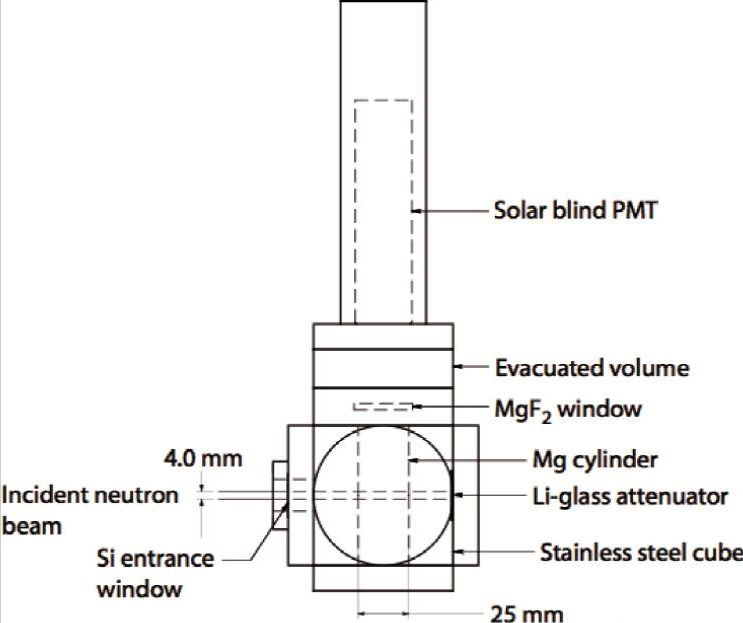
\includegraphics[scale=0.5]{lyman}\\
Рис.42 -- Чертеж экспериментальной ячейки:\\

Нейтроны попадают в цилиндрическую реакционную камеру диаметром 25 мм, где протоны и тритоны образуются в пучке диаметром менее 4 мм. Обнаруживаются альфа-фотоны Лаймана, которые проходят через окно MgF$_2$ в верхнем конце камеры. Однако, прежде чем попасть в цилиндр, нейтроны должны сначала пройти через «мертвое пространство» длиной $L_{dead}$, которое содержит гелий при том же давлении и ослабляется там, но никакие протоны или тритоны не попадают в цилиндр, и, следовательно, в мертвом теле не образуется излучение Лаймана-альфа. \\

Поток поглощенный в реакционной ячейке: \\

$I=I_0e^{-L_dead \sigma N}(1-e^{-d\sigma N})$, \\

где:\\
$I_0$ - входящий поток нейтронов, в приближении, что сечение поглощения в $^3 $He соответствует зависимости $1/v$\\
$\sigma$ - нейтронное сечение\\
$N$ - плотность атомов гелия в камере\\
$l_{dead} $ - длина мертвого пространства, в метрах
$d = 25$мм - диаметр реакционной камеры\\

Предполагалось, что все наблюдаемые фотоны генерируются внутри реакционной камеры и не имеют предпочтительного направления. 

Было получено соотношение между выходом фотонов и давлением, приведено на графике ниже:\\

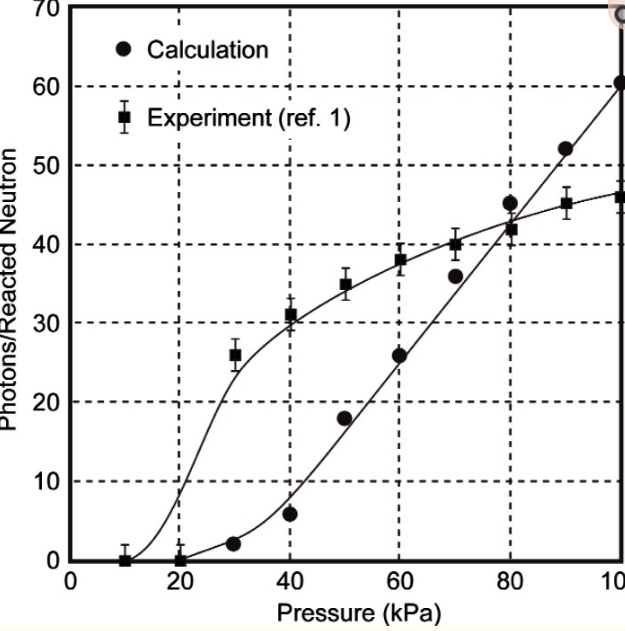
\includegraphics[scale=0.5]{lyman_p}\\
Рис.43 - соотношение между выходом фотонов и давлением \\

При более высоких давлениях можно ожидать, что количество наблюдаемых фотонов приблизится к предсказанию бесконечной среды в 154 фотона / нейтрон, поскольку все тритоны будут замедлены до 3 кэВ при более высоком давлении. \\

Было получено соотношение между количеством перезарядок и дистанцией пробега частиц, на графике ниже: \\

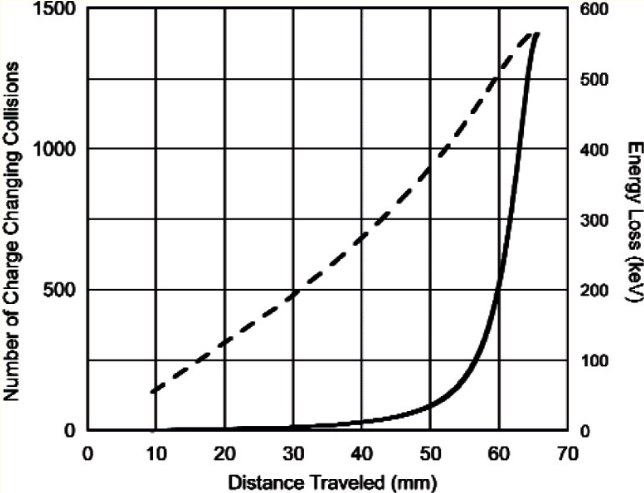
\includegraphics[scale=0.5]{lyman_x}\\
Рис.44 -- соотношение между количеством перезарядок и дистанцией пробега частиц \\

На основе данного эффекта создают мониторы по детектированию нейтронного излучения. В нашей работе, мы можем использовать данный эффект в качестве детектирования нейтронов для получения дифракционной картины, либо как источник фотонов.\\

\subsection{Эскиз}
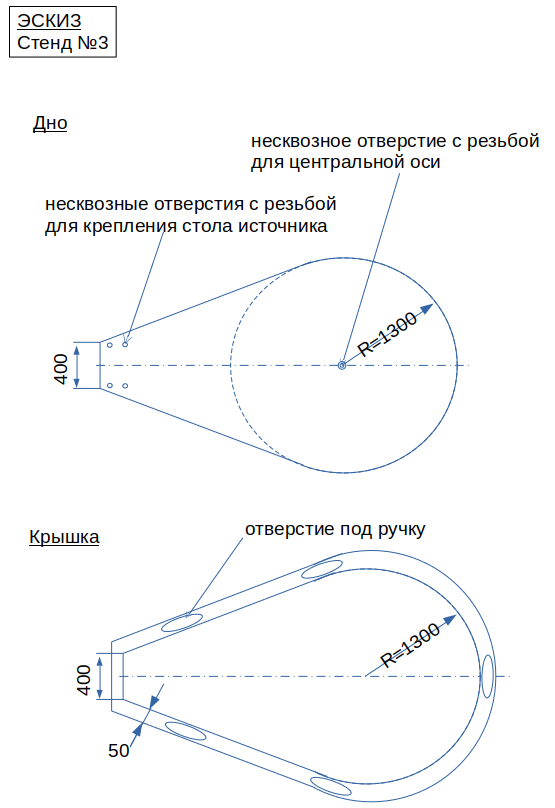
\includegraphics[scale=0.7]{stend_3_1}\\
Рис.45 - Эскиз Стенда №3 \\

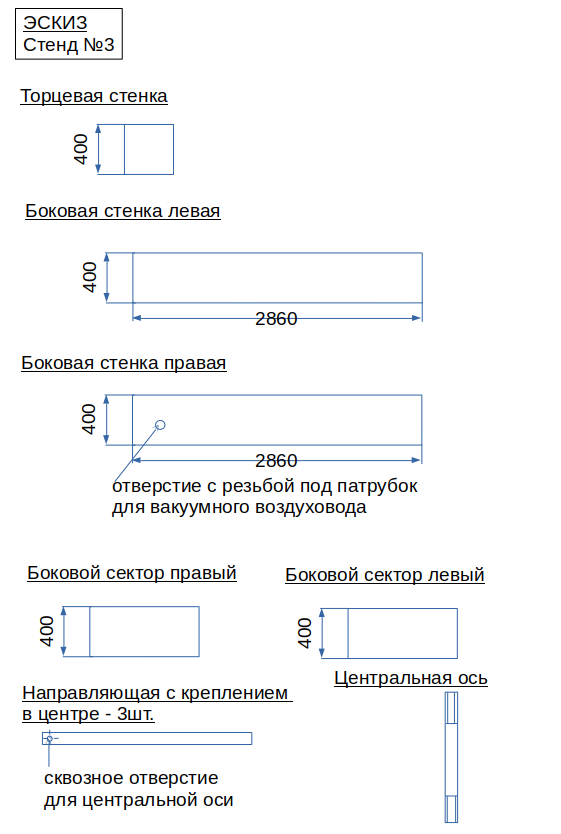
\includegraphics[scale=0.7]{stend_3_2}\\
Рис.46 - Эскиз Стенда №3 (продолжение)\\

\section{Экономический рассчет}
На момент написания были запрошены цены у производителей. \\

\subsection{Поставщик АО «В/О «Изотоп»}

\begin{tabular}{|p{5.5cm}|p{3.0cm}|p{3cm}|}
\hline
	Наименование & Количество & Стоимость, руб. \\
\hline
	AAm1.1.S2  & 2 & - \\
\hline
	НК248М11.44  & 2 & - \\
\hline	
	ОСГИ - Натрий-22  & 2 & - \\
\hline
	ОИДК Кобальт-60  & 2 & - \\
\hline
	ОРИБИ Стронций90+Иттрий-90  & 2 & - \\
\hline
	Итого:  & - & - \\
\hline
\end{tabular}


\subsection{Поставщик ООО «ЗАПАДПРИБОР»} 
\begin{tabular}{|p{5.5cm}|p{3.0cm}|p{3cm}|}
\hline
	Наименование & Количество & Стоимость, руб. \\
\hline
	ДКПО-Д-0,5-50  & 6 & - \\
\hline
	ДКПО-de/dx-25   & 6 & - \\
\hline	
	Д1А  & 6 & -\\
\hline
	СППД1  & 6 & -\\
\hline
	СКД1  & 6 & -\\
\hline
	Итого:  & - & - \\
\hline
\end{tabular}

\subsection{Поставщик Analog Devices} 
\begin{tabular}{|p{5.5cm}|p{3.0cm}|p{3cm}|}
\hline
	Наименование & Количество & Стоимость, USD \\
\hline
	AD8429BRZ  & 2 & 6.89 \\
\hline
	EVAL-INAMP-62RZ   & 2 & 40.23 \\
\hline	
\end{tabular}

\subsection{Поставщик MCUstore.ru} 
\begin{tabular}{|p{5.5cm}|p{3.0cm}|p{3cm}|}
\hline
	Наименование & Количество & Стоимость, руб \\
\hline
	Усилитель напряжения высокоточный AD620  & 2 & 594 \\
\hline
	Прочие радиодетали (сопротивления, конденсаторы, разъемы)   & - & 1000 \\
\hline	
	Mega 2560 CH340G Arduino совместимый контроллер с USB кабелем   & 2 & 732 \\
\hline	
\end{tabular}

\subsection{Поставщик metallsnab-nn.ru} 
\begin{tabular}{|p{5.5cm}|p{3.0cm}|p{3cm}|}
\hline
	Наименование & Количество,кг & Стоимость, руб/кг \\
\hline
	Плита алюминиевая АМГ6 100х1200х3000 ГОСТ 17232-99  & 500 & 383 \\
\hline
	Швеллер АМГ6 100х1200х3000 ГОСТ 17232-99  & 10 & 383 \\
\hline	
	Полоса алюминиевая 30х4 мм АД0   & 20 & 294 \\
\hline	
\end{tabular}

\subsection{Поставщик vseinstrumenti.ru} 
\begin{tabular}{|p{5.5cm}|p{3.0cm}|p{3cm}|}
\hline
	Наименование & Количество,кг & Стоимость, руб/кг \\
\hline
	Двухступенчатый шиберный высоковакуумный насос Rothenberger POАЭРBAK 170062  & 1 & 31943 \\
\hline
	Шланги , разъемы, муфты  & - & 5000 \\
\hline	
\end{tabular}


\subsection{Итоги рассмотрения} 
Без учета источников ИИ и датчиков, а также с использованием помещений и лабораторного оборудования,  производство стендов по материалам оценивается в районе 200 т.р.


\chapter{Варианты использования}
\section{Нейтронное излучение}
Основным источником нейтронов является ядерный реактор. Поэтому при построении квантового компьютера на  нейтронном излучении рационально разместить его в непосредственной близости от реактора, либо в самом реакторе. Строго говоря, сам реактор является большим квантовым компьютером с огромным количеством суперпозиций квантовых состояний. Для удобства оперирования с компьютером, можно сделать корпус в форме ТВС. \\
Отработанное ядерное топливо также является источником нейтронов и поэтому нейтронный компьютер возможно разместить в бассейне выдержки, либо в хранилище отработанного ядерного топлива. \\
Также возможно построение нейтронного компьютера на лабораторном источнике нейтронов, но тогда время работы компьютера будет ограничено сроком службы источника.\\

Для нейтронных квантовых компьютеров будет наблюдаться синергетический эффект в совместном использовании с ядерным реактором: нет необходимости в собственном источнике квантовых частиц, использование системы охлаждения реактора, совместное обслуживание реатора и компьютера.

\section{Альфа излучение}
К неоспоримым преимуществам квантового компьютера на альфа излучении является его относительная простота в организации радиационной защиты.\\
На рынке уже десятки лет присутствуют бытовые приборы, построенные на базе альфа излучения. Например к ним относятся датчики дыма HIS-07 и отечественные РИД-1. \\

Для альфа компьютеров возможен синергетический эффект с процессорами общего назначения, такими как Эльбрус. Возможно по аналогии с математическим сопроцессором выполнить достаточно компактный квантовый сопроцессор и использовать периферию и систему охлаждения самого компьютера. \\

\section{Излучение заряженных частиц}
У квантового компьютера на заряженных частицах есть одно важное преимущество - возможность работать на частицах без постороннего излучения. С помощью электромагнитных устройств можно отделить поток заряженных частиц от прочего фона излучения, что ценно для экспериментальной и исследовательской активности. Но также это влечет и основной недостаток - энергопотребление на инфраструктуру.

Такие квантовые компьютеры рационально строить совместно с ускорителями частиц, используя их инфраструктуру по управлению и разгону заряженных частиц.

\section{Гамма излучение}
Основная проблемма гамма излучения - относительно большая (по сравнению с альфа-излучением) радиационная защита. Источники гамма излучения давно используются в народном хозяйстве, но требуют отдельного помещения. Для разработки стационарных квантовых компьютеров этот факт может не являться ограничением.

\section{Адронные частицы}
Создание квантового компьютера на адронах даст большой ансамбль квантовых состояний, но на современный момент это достаточно экзотичный вариант, использования адронного коллайдера в качестве источника квантов для компьютера. Однако при всей фантастичности рассмотрим теоретические моменты. \\

Современная инженерия основывается при построении квантового компьютера на фотонах и достигла в этом значительных успехов, но посмотрим, откуда берутся фотоны и соответственно какими величинами мы оперируем. \\

Фотон - это бесструктурная фундаментальная частица, фундаментальный калибровочный базон, имеющий целочисленное внутренннее квантовое число спин $J=n\hbar , n=0,1, \dots $. Это квантовое число, а также пространственное положение используются в квантовых компьютерах. \\

Фотон отвечает за фундаментальное электромагнитное взаимодействие. \\

Рассмотрим происхождение фотонов - это квант энергии выделяющийся при переходе электрона в атоме с более энергетичного уровня (возбужденного), на основной (с меньшей энергией). \\

Рассмотрим объем в котором могут рождаться и поглащаться рассматриваемые фотоны:\\

$\lambdabar=\frac{\hbar}{T}= \frac{197meVfm}{8meV} \approx 25fm$ \\

Это теоретический предел в минимизации квантового компьютера на фотонах. \\

Рассмотрим, возможность уменьшения этого характерного линейного размера. Для этого попробуем перейти на другие квантовые объекты. \\

Представим вокруг себя сферу диаметром 10 км. Это наш современный квантовый компьютер. В этом объеме где-то перепрыгивает электрон в виде маленькой игрушечной машинки размером порядка 0,1мм с одного транспортного кольца на другое и при этом мигает фарами - испускает фотон.\\

Посмотрим, что еще есть в нашем мире - правильно, ядро, состоящее из нуклонов - в нашем масштабе это объекты порядка 10 см.\\ 

Хорошо бы было от 10км компьютера перейти к 10см - его уже можно носить в кармане.\\

Рассмотрим линейные размеры и способы взаимодействия:

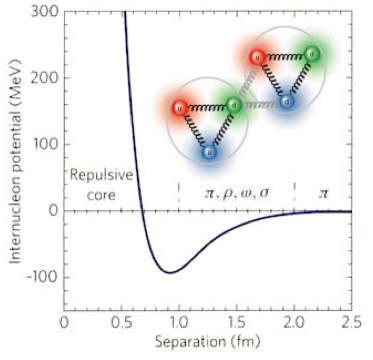
\includegraphics[scale=1]{ip} \\

Тезисно запишем ряд важных моментов:\\

Энергия связи на нуклон не зависит от размера ядра, нуклон взаимодействует только со своими ближайшими соседями.\\

Ядерная сила намного сильнее Кулоновской, но имеет отталкивающий компонент порядка 1фм. Это связано с существованием кварков внутри нуклона. Компонент отталкивания необходим для предотвращения слияния нуклонов. \\

Итак, мы имеем размер 1фм - за этой границей у нас кварки, обменивающиеся глюонами - фундаментальная частица сильного взаимодействия. Нуклоны между собой не могут обмениваться глюонами, они взаимодействуют друг с другом путем обмена мезонами, что и изображено на рисунке. \\

Заметим, что есть характерный размер 2фм и больше, где нуклоны обмениваются только пионами.\\

Получается, у нас есть новая перспективная частицу для нашего перспективного квантового компьютера - пион, который значительно уменьшит характерный размер, с 25 до 2фм. \\

Пионы самые легкие из мезонов частицы ~\cite{pion} :\\

 $\pi^{\pm } $ - 139.57039 $\pm$ 0.00018 МэВ (S=1.8)\\
 
 $\pi^0 $ - 134.9768 $\pm$ 0.0005 МэВ (S=1.1)\\
 
Моды распада: \\

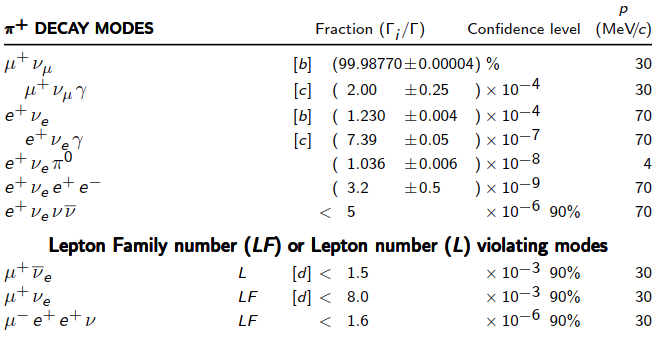
\includegraphics[scale=0.5]{decay_pp} \\

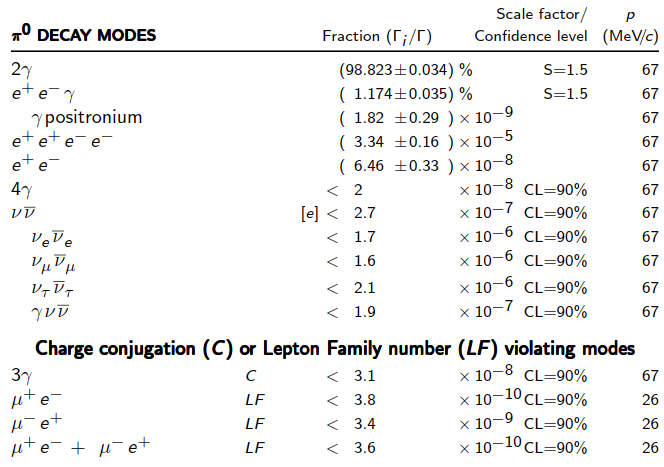
\includegraphics[scale=0.5]{decay_p0} \\

Получать измерения возможно по изменению квантовых векторов ядра, на котором ведется рассчет, либо другими коссвенными измерениями. На данный момент на этой частице видится предел по скорости смены состояний (минимальные размеры и минимальная масса), а значит максимум по скорости счета.\\

Возможно удастся теоретически обосновать создание квантовых операторов для фотонного компьютера на пионах/мюонах. Также, интересно рассмотреть и другие мезоны. \\

Данное направление далеко от инженерной активности, но перспективно с теоретической точки зрения.


\chapter{Компьютерное моделирование }
\section{Введение}
Для планируемых стендов было бы достаточным привести модель интерференции Маха-Зендера, но расширенный перечень моделей был приведен, чтобы продемонстрировать степень теоретической готовности к моделирования различных оптических систем и создать достаточный математический базис для дальнейших исследований. \\

Сурепозиция факторов: качественная картина (количество характерных линий) и количественные RGB-цвет и интенсивность будут являться результатом передаваемым от квантового компьютера на матрицу видео-камеры, подключенную через цифровой интерфейс(USB) к классическому компьютеру. Понятно, что USB интерфейс, также как и другие интерфейсы компьютера работают на определенных частотах и имеют ограничивающую их пропускную способность, но для прототипирования подобный интерфейс является достаточным.\\

Сразу видим разницу между классическими и кванотовыми компьютерами. В квантовом компьютере мы всегда возвращаем картину - матрицу в RGBa формате. \\

Физика картин была рассмотренав разделе физических основ квантовых вычислений, а здесь мы приводим результаты численного моделирования.\\

Моделирование было произведено ня языке Python с использованием opensource библиотек: matplotlib, tk, lightpipe \\

Схемы установок взяты из ~\cite{optic}

\section{Дифракция - плоская волна, круглое отверстие, вар. 1}
\subsection{Модель}
\includegraphics[scale=0.5]{model/Difraction/setup}\\
Рис.47 -- Модель Дифракция - плоская волна, круглое отверстие, вар. 1\\

\subsection{Картина}
\includegraphics[scale=0.5]{model/Difraction/image}\\
Рис.48 -- Картина Дифракция - плоская волна, круглое отверстие, вар. 1\\

\subsection{Исходный код}
Исходный код размещен в открытом доступе на GitHub: \url{https://github.com/juhnowski/qc_Diffraction.git}


\section{Дифракция Френеля - плоская волна, круглое отверстие, вар. 2}
\subsection{Модель}
\includegraphics[scale=0.5]{model/Frenel/FresnelPlaneSetup}\\
Рис.49 -- Модель Дифракция - плоская волна, круглое отверстие, вар. 2\\

Картины были рассчитаны при переменном $z$ и апертуре $d=1$мм
\subsection{Картина}
\begin{tabular}{|p{3,7cm}|p{3,7cm}|p{3,7cm}|p{3,7cm}|}
\hline
	$z=0,01$см & $z=1,20$см & $z=4,77$см & $z=10,72$см\\
	\includegraphics[scale=0.2]{model/Frenel/00_01}  & \includegraphics[scale=0.2]{model/Frenel/01_20} & 	\includegraphics[scale=0.2]{model/Frenel/04_77} & \includegraphics[scale=0.2]{model/Frenel/10_72}\\
\hline
	$z=11,91$см & $z=13,10$см & $z=14,29$см & $z=15,49$см\\
	\includegraphics[scale=0.2]{model/Frenel/11_91}  & \includegraphics[scale=0.2]{model/Frenel/13_10} & 	\includegraphics[scale=0.2]{model/Frenel/14_29} & \includegraphics[scale=0.2]{model/Frenel/15_49}\\
\hline
\end{tabular}
Рис.50 -- Картина Дифракция - плоская волна, круглое отверстие, вар. 2\\

\subsection{Исходный код}
Исходный код размещен в открытом доступе на GitHub: \url{https://github.com/juhnowski/qc_Frenel}

\section{Дифракция Френеля - сферическая волна, круглое отверстие}
\subsection{Модель}
\includegraphics[scale=0.5]{model/FrenelSphere/FresnelSphericalSetup}\\
Рис.51 -- Модель Дифракция Френеля - сферическая волна, круглое отверстие \\

Картины были рассчитаны при переменной $z_2 $ и постоянных: $z_1 = 50$см и апертуре $d=1$мм
\subsection{Картина}
\begin{tabular}{|p{3,7cm}|p{3,7cm}|p{3,7cm}|p{3,7cm}|}
\hline
	$z_2=4$см & $z_2=50$см & $z_2=100$см & $z_2=150$см \\
	\includegraphics[scale=0.2]{model/FrenelSphere/50_04}  & \includegraphics[scale=0.2]{model/FrenelSphere/50_50} & 	\includegraphics[scale=0.2]{model/FrenelSphere/50_100} & \includegraphics[scale=0.2]{model/FrenelSphere/50_150}\\
\hline
\end{tabular}
Рис.52 -- Картина Дифракция Френеля - сферическая волна, круглое отверстие  \\

\subsection{Исходный код}
Исходный код размещен в открытом доступе на GitHub: \url{https://github.com/juhnowski/qc_Fresnel_s}\\

\section{Внутреннее отражение и преломление}
\subsection{Модель}
\includegraphics[scale=0.7]{model/ReflectRefract/ReflectSetup}\\
Рис.53 -- Модель Внутреннее отражение и преломление \\

Картины были получены для постоянного поляризационного угла $\phi_in = 79$град и переменного $\phi_t$, где первый ряд - отраженный поток, второй - преломленный
\subsection{Картина}
\begin{tabular}{|p{3,7cm}|p{3,7cm}|p{3,7cm}|p{3,7cm}|}
\hline
	$\phi_t=32,14$град  & $\phi_t=37,50$град & $\phi_t=40$град & $z_2=41,25$см \\
	\includegraphics[scale=0.4]{model/ReflectRefract/r_32_14}  & \includegraphics[scale=0.4]{model/ReflectRefract/r_37_50} & 	\includegraphics[scale=0.4]{model/ReflectRefract/r_40} & \includegraphics[scale=0.4]{model/ReflectRefract/r_41_25} \\

\includegraphics[scale=0.4]{model/ReflectRefract/t_32_14}  & \includegraphics[scale=0.4]{model/ReflectRefract/t_37_50} & 	\includegraphics[scale=0.4]{model/ReflectRefract/t_40} & \includegraphics[scale=0.4]{model/ReflectRefract/t_41_25} \\

\hline
\end{tabular}
Рис.54 -- Картина Внутреннее отражение и преломление \\

\subsection{Исходный код}
Исходный код размещен в открытом доступе на GitHub: \url{https://github.com/juhnowski/qc_ReflectRefract}\\

\section{Эксперимент Юнга}
\subsection{Модель}
\includegraphics[scale=0.7]{model/Yung/twoholessetup}\\
Рис.55 -- Модель Эксперимент Юнга \\

\subsection{Картина}
\includegraphics[scale=0.4]{model/Yung/young} \\
Рис.56 -- Картина Эксперимент Юнга \\

\subsection{Исходный код}
Исходный код размещен в открытом доступе на GitHub: \url{https://github.com/juhnowski/qc_Yung}\\

\section{Моды Эрмита-Гаусса}
\subsection{Модель}
Гауссов пучок — пучок электромагнитного излучения, в котором распределение электрического поля и излучения в поперечном сечении хорошо аппроксимируется функцией Гаусса. Когерентный световой пучок с гауссовым распределением поля имеет фундаментальное значение в теории волновых пучков. Этот пучок называют основной модой в отличие от других мод более высокого порядка.
\subsection{Картина}
\includegraphics[scale=0.4]{model/Gauss/hg_laser_mode} \\
Рис.57 -- Картина Моды Эрмита-Гаусса \\

\subsection{Исходный код}
Исходный код размещен в открытом доступе на GitHub: \url{https://github.com/juhnowski/qc_Gauss}\\

\section{Моды Лагерра-Гаусса}
\subsection{Картина}
\includegraphics[scale=0.6]{model/Gauss/Gauss_laser_mode_LG} \\
Рис.58 -- Картина Моды Лагерра-Гаусса
\subsection{Исходный код}
Исходный код размещен в открытом доступе на GitHub: \url{https://github.com/juhnowski/qc_Gauss}\\

\section{Множественные прорези}
\subsection{Модель}
В этом примере мы демонстрируем использование щелей в ряд. Таким способом можно сделать решетку. В пучке есть две длины волны, что демонстрирует использование решетки в качестве спектрометра. Интенсивности двух полей можно просто сложить после раздельного распространения.
Экран: \\
\includegraphics[scale=0.7]{model/MultiSlits/screen} \\
Рис.59 -- Экран модели Множественные прорези \\
\subsection{Картина}
\includegraphics[scale=1]{model/MultiSlits/image} \\
Рис.60 -- Картина модели Множественные прорези \\
\subsection{Исходный код}
Исходный код размещен в открытом доступе на GitHub: \url{https://github.com/juhnowski/qc_MultiSlit}\\

\section{Множественные отверстия}
\subsection{Модель}
В этом примере мы демонстрируем использование ряда отверстий. Таким способом можно сделать решетку. В пучке есть две длины волны, что демонстрирует использование решетки в качестве спектрометра. Интенсивности двух полей можно просто сложить после раздельного распространения.
Экран: \\
\includegraphics[scale=0.7]{model/MultiHole/screen} \\
Рис.61 -- Экран модели Множественные отверстия \\
\subsection{Картина}
\includegraphics[scale=0.7]{model/MultiHole/intencity} \\
Рис.62 -- Картина модели Множественные отверстия \\
\subsection{Исходный код}
Исходный код размещен в открытом доступе на GitHub: \url{https://github.com/juhnowski/qc_MultiHole}\\

\section{Датчик Шака Хартмана}
\subsection{Модель}
Датчик Шака Хартмана - это прибор для измерения фазового распределения волнового фронта.\\
Экран:\\
\includegraphics[scale=0.7]{model/ShackHartman/plane_screen} \\
Рис.63 -- Модель Шака Хартмана \\
\subsection{Картина}

\includegraphics[scale=0.3]{model/ShackHartman/defocus} \\
Рис. 64 -- Картина с аберрацией Зернике-дефокусировки \\

\includegraphics[scale=0.3]{model/ShackHartman/vert} \\
Рис. 65 -- При аберрации вертикальной \\
\subsection{Исходный код}
Исходный код размещен в открытом доступе на GitHub: \url{https://github.com/juhnowski/qc_MultiHole}\\


\section{Две непараллельные прорези, вер.1}
\subsection{Модель}
Экран:\\
\includegraphics[scale=0.3]{model/TwoSlitsTilts/plane} \\
Рис.66 -- Модель Две непараллельные прорези, вер.1 \\
\subsection{Картина}
\includegraphics[scale=0.3]{model/TwoSlitsTilts/intencity} \\
Рис.67 -- Картина Две непараллельные прорези, вер.1 \\
\subsection{Исходный код}
Исходный код размещен в открытом доступе на GitHub: \url{https://github.com/juhnowski/qc_TwoSlitsTilts}\\

\section{Две непараллельные прорези, вер.2}
\subsection{Модель}
Экран:\\
\includegraphics[scale=0.3]{model/TwoSlitsTilts2/plane_screen}\\
Рис.68 -- Модель Две непараллельные прорези, вер.2 \\
\subsection{Картина}
\includegraphics[scale=0.3]{model/TwoSlitsTilts2/intencity} \\
Рис.69 -- Модель Две непараллельные прорези, вер.2 \\
\subsection{Исходный код}
Исходный код размещен в открытом доступе на GitHub: \url{https://github.com/juhnowski/qc_TwoSlitsTilts2}\\

\section{Интерферометр Маха-Зендера}
\subsection{Картина}
\includegraphics[scale=0.3]{model/MachZender/image} \\
Рис.70 -- Картина Интерферометр Маха-Зендера
\subsection{Исходный код}
Исходный код размещен в открытом доступе на GitHub: \url{https://github.com/juhnowski/qc_MachZender}\\


\section{Заключение}
В заключении этой главы, стоит отметить, что был продемонстрирован достаточно богатый инструмент для моделирования волновых эффектов. Поскольку квантовые объекты представляются волновыми функциям, то мы теоретически может вычислить конфигурации различных оптических систем и сравнить их с экспериментальными результатами. Причем, не стоит игнорировать шум ~\cite{noise} , поскольку в нем могут скрываться характерные картины, которые мы не смоделировали и тем самым, поправить математическую модель.

\chapter{Подведение итогов}

\section{Результаты исследования}
Были рассмотрены:\\

-- альфа-частицы - возможность использования в мобильных, персональных устройствах;\\

-- нейтроны - реакторная инфраструктура (реактор, биологическая защита, бассейн выдержки, хранилище отработанного ядерного топлива) \\

-- заряженные частицы - реакторная инфраструктура, лаборатории для работы с источниками ионизационного излучения\\

-- гамма излучение - как полезная нагрузка в инфраструктуре гамма-лазера \\

Были построены компьютерные модели, численно моделирующие интерференционные картины \\

Теоретически была продемонстрирована возможность создания квантового компьютера на частицах ядерного реактора. \\

Были приведены варианты построения квантового компьютера на различных частицах и возможные варианты использования. \\

Предложены лабораторные стенды для прототипирования квантовых компьютерах на различных частицах. \\

Подготовлены для дальнейшей инженерной работы основные теоретические зависимости и компьютерные модели.

\section{Выводы}
По результатам проведенной исследовательской работы, можно заключить следующие выводы: \\

1. На частицах источников ионизирующего излучения возможно построение квантовых операторов, а значит и квантового компьютера.\\


2. Возможна минимизация квантового компьютера за счет применения альфа-излучения.\\

3. Возможна минимизация энергопотребления квантового компьютера -  так как источники излучения не потребляют энергии из вне, а процессы не требуют улюбокого охлаждения. \\

4. Когерентность источника не является обязательной, поскольку квантовый алгоритм Дойча работает на одном кванте. \\ 

5. Перспективно рассмотреть возможность квантового компьютера на ускорителях, поскольку некоторые эффекты (например радужное сияние), требуют разгона частиц. Также, на ускорителях мы можем изучить возможность построения квантовых компьютеров на фундаментальных частицах и их производных. В этом случае мы существенн расширим ансамбль квантовых состояний, а знгачит и кубитность. \\

6. Перспективна работа над эскизным проектом нейтронного квантового компьютера, в формфакторе ТВС для интеграции с экосистемой ядерного топливного цикла(Ядерный реактор, бассейн выдердки, хранилище отработанного ядерного топлива)\\

7. Перспективна работа над эскизным проектом альфа квантового компьютера, в качестве сопроцессора МЦСТ "Эльбрус"\\

8. Перспективна работа над эскизным проектом гамма квантового компьютера, особенно при появлении в перспективе гамма-лазера\\

9. Перспективна работа над эскизным проектом квантового компьютера на заряженных частицах, в формфакторе ТВС \\

10. Перспективна работа над эскизным проектом интерфейсов передачи результатов рассчетов от квантового компьютера классическому на основе эффекта Лаймона при использовании Гелий-3. \\

11. Для экспериментального подтверждение теоретических выводов необходимо получение гранта, средства которого пойдут на построение стендов (1 млн.руб.), закупку расходников, заработную плату.



\begin{thebibliography}{3}
\bibitem{Courcera_KvVich}
Сысоев С.С., Санкт-Петербургский государственный университет ---  Квантовые вычисления (Quantum computing) --- https://www.coursera.org/learn/kvantovyye-vychisleniya --- 2020, 
\bibitem{Courcera_NPh}
Martin Pohl, Anna Sfyrla, Mercedes Paniccia, Университет Женевы --- Particle Physics: an Introduction. --- https://www.coursera.org/learn/particle-physics/ --- 2020
\bibitem{Lymon_1}
Alan K. Thompson, Michael A. Coplan, John W. Cooper, Patrick P. Hughes, Robert E. Vest, Charles Clark  --- Observation of the $^3 $He(n, tp) Reaction by Detection of Far-Ultraviolet Radiation https://www.ncbi.nlm.nih.gov/pmc/articles/PMC4654066/ Published online 2008 Apr 1. doi: 10.6028/jres.113.006
\bibitem{Lymon_2}
Alan K. Thompson, Michael A. Coplan, John W. Cooper, Patrick P. Hughes, Robert E. Vest, Charles Clark   ---The Detection of Lyman Alpha Radiation Formed by the Slowing Down of Protons and Tritons Produced by the 3He (n, tp) Reaction—A Model Study https://www.ncbi.nlm.nih.gov/pmc/articles/PMC4646570/ --- Published online 2009 Jun 1. doi: 10.6028/jres.114.012
\bibitem{Opt}
А.И.Хизер, Ю.А.Бережной, В.В.Пилипенко --- Квантовая интерференция и ядерная оптика -- 2000, Харьковский государственный университет, Харьков, Украина
\bibitem{shirokov}
Широков Ю. М., Юдин Н. П. Ядерная физика. --- М.: Наука, 1972. --- 670 с.
\bibitem{rffi_o_216479}
Воронин В.В. Нейтронная оптика и динамическая дифракция нейтронов в кристаллах без центра симметрии. - РФФИ -- 2002г. Номер гранта 02-02-17042 
\bibitem{ng_1}
Д.А.Кузьмин, Ю.А.Толмачёв Форма аппаратной функции процедуры восстановления изображения точечного объекта в нейтронной голографии по схеме внутреннего источника -- Вестник Санкт-Петербургского университета -- Сер.4 2009 Вып.1, стр.18-26 
\bibitem{ng_2}
Sur B., Rogge R. B., Hammond R. P., Anghel V. N. P., Katsaras J.Atomic structureholography using thermal neutrons // Nature. 2001. Vol. 414. P. 525–527.
\bibitem{ng_3}
Пастор А. А., Толмачёв Ю. А., Шарков И. Г.Опознавание образов как метод анализа голограмм сложных молекул // Вестн. С.-Петерб. ун-та. Сер. 4: Физика, химия. Вып. 1. 2004.С. 82–90.
\bibitem{optic}
Frank L Pedrotti, Leno M Pedrotti , Leno S Pedrotti Introduction to Optics (3rd Edition) -- Pearson; 3rd Edition (April 17, 2006)
\bibitem{wiki}
Котляр В. В., Алмазов А. А., Хонина С. Н. ЭЛЛИПТИЧЕСКИЙ СВЕТОВОЙ ПУЧОК ГАУССА-ЛАГЕРРА --  Институт систем обработки изображений РАН, Самарский государственный аэрокосмический университет -- 2005
\bibitem{noise}
Philip Ball Putting quantum noise to work -- \url{https://physicsworld.com/a/putting-quantum-noise-to-work/} -- 18 Sep 2018
\bibitem{qbit}
\url{https://www.kaggle.com/ashishpatel26/quantum-computing-introduction-using-python}
\bibitem{bloch}
Соловьев Владимир Михайлович КВАНТОВЫЕ КОМПЬЮТЕРЫ И КВАНТОВЫЕ АЛГОРИТМЫ. Часть 1. КВАНТОВЫЕ КОМПЬЮТЕРЫ ---  Известия Саратовского университета -- 2015
\bibitem{saricheva}
Л.И.Сарычева Введение в физику микромира. Физика частиц и ядер. -- URSS, М.-2012
\bibitem{bogdanov}
Bogdanov U. I., Kokin A. A., Lukichev V. F., Orlikovskij A. A., Semenihin I. A., Chernavskij A. U. -- Quantum mechanics and the development of information technology.Information technologies andcomputer systems, 2012, no. 1, pp. 17–31 (in Rus-sian) Closing   in   on   quantum   computing. \url{http://www.wired.com/2014/10/quantum-computing-close (accessed 23, June, 2015)}
\bibitem{lloyd}
Lloyd S. Programming universe. A quantum computer science and the future. Мoscow, Alpina non-fiction, 2014
\bibitem{Valiev}
Valiev K. A. Quantum computers and quantumcomputing.Successes of physical sciences, 2005,vol. 175, no. 1
\bibitem{Smale}
Smale S. On the problems of computational com-plexity. Mathematical education. Мoscow, MCN-TO, 2000, Ser. 3, iss. 4, pp. 115–119.
\bibitem{Shor}
Shor P. W.Polynomial-Time Algorithms for PrimeFactorization and Discrete Logarithms on a Quantum  Computer.  1996.  arXiv:  quant-ph/9508027.28 p.
\bibitem{Nielsen}
Nielsen M., Chuang I.Quantum Computation andQuantum Information. 10th Anniversary Edition.Cambridge Univ. Press, 2010, 698 p.
\bibitem{Rieffe}
Rieffe E. G., Polak W. H.Quantum computing:a gentle introduction. Scientific and EngineeringComputation. MIT Press, 2011, 389 p.
\bibitem{Belinskij}
Belinskij A. V. Quantum nonlocality and the ab-sence of a priori values for measurable quantitiesin experiments with photons.Successes of physicalsciences, 2003, vol. 173, no. 8, pp. 905–909.
\bibitem{Bouwmeester}
Bouwmeester  D.,  Ekert  F.,  Zeilinger  A.ThePhysics of Quantum Information. Springer, 2000,315 p.
\bibitem{Menskij}
Menskij M. B.Quantum measurement and deco-herence. Models and phenomenology: Trans. fromEnglish. Мoscow, Fizmatlit, 2001, 232 p.
\bibitem{Preskill}
Preskill  J. Quantum  information  and  quantumcomputation. Vol. 2.Мoscow, Izhevsk, SIC «Reg-ular and Chaotic Dynamics», Institute of ComputerScience, 2011, 312 p.
\bibitem{algalg}
Algebraic  and  Number  Theoretic  Algorithms.Available at: http://math.nist.gov/ quantum/zoo/(accessed 23, June, 2015).
\bibitem{Venegas}
Venegas-Andraca S. E.Quantum Walks for Com-puter Scientists. Synthesis Lectures on QuantumComputing. Morgan Claypool, 2008, 133 p.
\bibitem{Kastrenakes}
Kastrenakes  Jacob.  Researchers  smash  throughquantum computer storage record. Available at:http://www.theverge.com/2013/11/14/5104668/qubits-stored-for-39 - minutes - quantum - computer-new-record (accessed 23, June, 2015).
\bibitem{Kelly}
Kelly J. State preservation by repetitive error detec-tion in a superconducting quantum circuit.Nature,Macmillan Publ. Ltd., 2015, vol. 519, pp. 66–69.Информатика477
\bibitem{pion}
P.A.Zylaet al.(Particle Data Group), Prog. Theor. Exp. Phys.2020, 083C01 (2020)

\end{thebibliography}

\end{document}


